% WIP-Stil LaTeX-Vorlage für (englischsprachige) Abschluss- und Studienarbeiten

\documentclass[
	11pt,								% Schriftgroesse
	DIV10,								% Koma-Script-Klassen: Groesse des bedruckbaren Bereichs
	a4paper,         					% Format
	oneside,							% Einseitiges Dokument
	headheight=20pt,					% Höhe Dokumentenkopf
	footheight=20pt,					% Höhe Dokumentenfuß
    parskip=full,						% Abstand zwischen Absaetzen (ganze Zeile)
    listof=totoc,						% Verzeichnisse im Inhaltsverzeichnis aufführen
	bibliography=totoc,					% Literaturverzeichnis im Inhaltsverzeichnis aufführen
	index=totoc,						% Index im Inhaltsverzeichnis aufführen
	%final
    %draft								% Status des Dokuments
]{scrartcl}

%%% Schrift %%%
\usepackage[utf8]{inputenc}				% Umlaute im Tex-Code erlauben
\usepackage[T1]{fontenc}
\usepackage[ngerman, english]{babel}	% Sprachpaket Deutsch
\usepackage[useregional]{datetime2}
\selectlanguage{english}
\usepackage{csquotes}					% Zitation im gleichen Stil 
\renewcommand{\baselinestretch}{1.50}	% Zeilenabstand 1.5
\normalsize
%\usepackage{uarial}						% Schriftart Arial, kann ausdokumentiert werden, wenn die Standardschrift benutzt werden soll
\renewcommand{\familydefault}{\sfdefault}
\usepackage{blindtext}					% zum Testen des Layouts
\usepackage{microtype}					% Verbesserter Randausgleich
\usepackage{color}
\usepackage{eurosym} 					% Eurozeichen
\usepackage{xcolor}
\usepackage{datetime}
\usepackage{dcolumn}
\usepackage{todonotes}
\usepackage{eurosym}
\usepackage{amssymb}

%%% Anpassung des Formats %%%
\RedeclareSectionCommand[
  beforeskip=-1sp,						% minimaler Abstand nach Überschrift, anschließend nicht einrücken
  afterskip=1sp]{section}
\RedeclareSectionCommand[
  beforeskip=-1sp,						% siehe oben 
  afterskip=1sp]{subsection}
\RedeclareSectionCommand[
 beforeskip=-1sp,						% siehe oben
  afterskip=1sp]{subsubsection}
\RedeclareSectionCommand[
  beforeskip=-1sp,						% siehe oben
  afterskip=1sp]{paragraph}
\RedeclareSectionCommand[
 beforeskip=-1sp,						% siehe oben
 afterskip=1sp]{subparagraph}

%%% Änderungen des Inhaltsverzeichnis %%%
\usepackage[titles]{tocloft}			% wird zur Änderung des toc verwendet

\renewcommand{\cftsecleader}			% führe Punkte im toc auch für sections ein, Punkte fetter als normal
	{\bfseries\cftdotfill{\cftdotsep}}
\renewcommand{\cftdotsep}{0.1}			% setze Punkteabstand enger	

%%% definiere Inhaltsübersicht %%%
% Achtung: In Vorlage auskommentiert %
\newcommand*\inhaltsuebersicht{%
\section*{Content Overview}				% Name 
\begingroup
\value{tocdepth}\shorttocdepth\relax
\makeatletter
\input{\jobname.toc}
\makeatother
\endgroup
}
\newcommand*{\shorttocdepth}{1}			% Tiefe der Inhaltsübersicht == 2

%%% Bilder %%%
\usepackage{graphicx}
\graphicspath{{./Bilder/}}				% Bilderverzeichnis
\usepackage{overpic} 					% Beschriftung in Abbildung platzieren
\usepackage{here}						% Bildplatzierung mit [H]

%%% Verschiedenes, Mathe-Funktionen, Layout %%%
\usepackage{float,caption}
\usepackage{amsmath,amsfonts}
\usepackage{mathtools}
\usepackage{amssymb}
\usepackage{exscale}
\usepackage[normalem]{ulem}
\usepackage{setspace}
\usepackage[a4paper,
    lmargin={2.5cm},
    rmargin={2.5cm},
    tmargin={2cm},
    bmargin={2cm}
    ]{geometry}
    
\addtolength{\footskip}{-0.5cm}			% Fussbereich 0.5cm höher, sodass die Seitennummierung höher ist

%%% Listen %%%
%\usepackage{enumitem}
\usepackage{paralist}					% Für kompakte Listen
\setlength{\pltopsep}{5pt}				% setzt den oberen Abstand der compactitem- und compactenum-Liste auf eine Zeilenbreite

%%% Tabellen %%%
\usepackage{tabularx}
\usepackage{booktabs}					% Platzverschwendung in Tabellen vermeiden
\usepackage{array}						% mehr Möglichkeiten der Darstellung

%%% Kopf und Fußzeile %%%
\usepackage[nouppercase,headsepline]{scrpage2}
\pagestyle{scrheadings}
\clearscrheadfoot
%\chead{\textit{TU Berlin, Fachgebiet Wirtschafts- und Infrastrukturpolitik (WIP)}}
	% Leerzeichen zwischen FN-Nummer und FN-Text
\deffootnote[]{1.5em}{1em}{\textsuperscript{\thefootnotemark}\enskip}
\cfoot{\normalsize{\emph{\thepage}}}

%%% URL's %%%
\usepackage[lowtilde]{url}				% bei Verwendung eines Tildezeichens wird es normal gesetzt
\urlstyle{same}
\usepackage{etoolbox}

%%% Zitation %%%
\usepackage[style=chicago-authordate,
			%style=authoryear,
			%style=chicago,
            giveninits,					% Vornamen abkürzen
			maxbibnames=10,				% in der Bib werden 10 Autoren ausgegeben (bis zu 10)
            maxcitenames=2,				% max. 3 Autoren bei \cite
            backend=biber,
			doi=false,
			isbn=false,
			url=false,
            natbib=true,				% verwendet Natbib 
            sorting=nyt					
			]{biblatex}

\addbibresource{microgrid_literature.bib}
\addbibresource{extra_literature.bib}
\usepackage{breakcites}

\DeclareNameAlias{author}{last-first}				

% *****************************************
%%% Anpassungen für englische Literatur %%%
% *****************************************

\DeclareFieldFormat[article]{title}{"#1\adddot"}				
\DeclareFieldFormat[inproceedings]{title}{"#1\addcomma"}				
%\DeclareFieldFormat[book]{title}\textit{{#1}\isdot}    			
\DeclareFieldFormat[techreport]{title}{"#1\adddot"}					
\DeclareFieldFormat[incollection]{title}{"#1\adddot"} 
\DeclareFieldFormat[online]{title}{#1\isdot}           		
\DeclareFieldFormat[misc]{title}{"#1\isdot"}					

\DeclareFieldFormat[inproceedings]{booktitle}{proceedings of #1}	

\AtEveryBibitem{\clearlist{language}}

\AtEveryBibitem{%
	\ifentrytype{online}
	{}
	{\clearfield{urlyear}\clearfield{urlmonth}\clearfield{urlday}}}

\AtEveryBibitem{%
	{\clearfield{month}\clearfield{day}}}

\DefineBibliographyStrings{english}{andothers = {et\,al\adddot}}

\DeclareFieldFormat[article]{number}{#1}					
\DeclareFieldFormat[article]{pages}{\space#1}

\usepackage{xpatch}
\xpretobibmacro{author}{\mkbibbold\bgroup}{}{}					% Autor fett
\xapptobibmacro{author}{\egroup}{}{}

\DeclareSourcemap{
	\maps{\map{
			\step[fieldsource=language, fieldset=langid, origfieldval, final]
			\step[fieldset=language, null]}}}

\usepackage[pdfborder={0 0 0},								% Rahmen in pdf nicht sichtbar
			breaklinks=true,
            %draft,											% alle Links abschalten
            ]{hyperref}

%%%%%%%%%%%%%%%%%%%%%%%%%%%%%%%%%%%%%%%%%%%%%%%%%%%%%%%%%%%%%%%%%%%%%%%%%%%%%%%%%%%%%%%%%%%%%%%
% Beginn des Dokument

% *************************************
%%% HIER DIE TITELSEITE BEARBEITEN %%%%
% *************************************

%%% Titelseite %%%
\newcommand{\autor}{Maximilian Eißler} 		% Name des Autors
\newcommand{\matriculation}{374881} 
\newcommand{\mailaddress}{eissler@campus.tu-berlin.de}

\newcommand{\betreuer}{Dr. Pao-Yu Oei} 		% Namen der Betreuer
\newcommand{\betreuerzwei}{Thorsten Burandt}
                      
                  
%\newcommand{\datum}{\selectlanguage{ngerman}\today}
\newcommand{\engdate}{\selectlanguage{english}\today}

%%% Glossar und Abkürzungsverzeichnis %%% 
\usepackage[acronym,
            nonumberlist,									% keine Seitenzahlen anführen
            toc,											% im Inhaltsverz. mit aufnehmen
            style=super,									% Einträge mit Abstand setzten 
            nopostdot,										% kein schließender Punkt
           	nogroupskip]									% kein Absatz zwischen Gruppen
           	{glossaries}									% muss nach \usepackage{hyperref} geladen werden, damit auch Einträge des Abkürzungsverzeichnisses verlinkt sind
\makeglossaries

%***********************************
%%% HIER DIE AKRONYME DEFINIEREN %%%
%***********************************

%%% exempl. Akronyme %%%
\newacronym[firstplural=renewable energy sources (RES)]{res}{RES}{renewable energy sources}
\newacronym{eeg}{EEG}{Erneuerbare-Energien-Gesetz}
\newacronym{tso}{TSO}{Transmission System Operator}
\newacronym{rmse}{RMSE}{root-mean squared error}
\newacronym{gams}{GAMS}{General Algebraic Modeling System}
\newacronym[firstplural=Energiewirtschaftsgesetzes (EnWG)]{enwg}{EnWG}{Energiewirtschaftsgesetz}
\newacronym{ihv}{i.H.v.}{in Höhe von}
\newacronym[firstplural=Millimetern (mm)]{mm}{mm}{Millimeter}
\newacronym[firstplural=Off\-shore-Wind\-parks (OWP)]{owp}{OWP}{Off\-shore-Wind\-park}
	% sort= ermöglicht korrekte Sortierung von Umlauten
\newacronym[sort=uebertr]{unb}{\"UNB}{Übertragungsnetzbetreiber}

% ***********************************************************************************
% Beginn des Dokuments
% ***********************************************************************************

\begin{document}\selectlanguage{english}
% ***********************************************************************************
% Automatische Zusammensetzung der Titelseite, nur aendern, falls noetig!
% ***********************************************************************************

	\thispagestyle{plain}
	\begin{titlepage}
		\vspace{0cm} 
		\begin{center}
			
\includegraphics[width=2.5cm]{pictures/TU_Logo_kurz_4c_rot}\\
			\normalsize{Technische Universität Berlin}\\
			Fakultät VII Wirtschaft \& Management\\
			Fachgebiet Wirtschafts- und Infrastrukturpolitik (WIP)
		\end{center}
        \vfill
		%\vspace*{\fill}
		\begin{center}
			%\Large{\textbf{\textsc{\doctitle}}}\\
			\Large{\textbf{Bachelorarbeit}}\\
            \LARGE{\textbf{An Open-Source Optimization Tool for \\  Microgrid Energy Systems}}\\[2ex]            
			\vfill
			
% "Ockerfarbener Kasten":

%{
%\setlength{\fboxrule}{0.2mm}
%\definecolor{ocker}{RGB}{196,188,150}
%			\selectlanguage{ngerman}\normalsize
%\fcolorbox{black}{ocker}{\begin{minipage}{\textwidth}

%\textbf{Dateinamen-Kern (mit Versions-Nr. 000):} 
%\url{vorlage_latex_v000}

%\textbf{Ablage-Server-Pfad (fixiert):} 
%\url{Z:\\lehre\\BEREICH_WIPOL_ETC\\veranstaltung___ewa_seminar\\_formatvorlagen\\LaTeX-Vorlagen\\Standard}

%\textbf{Aktueller Ablageort:} \url{\\\\afs\\tu-berlin.de\\units\\Fak_VII\\wip\\share\\lehre\\BEREICH_WIPOL_ETC\\veranstaltung___ewa_seminar\\_formatvorlagen\\LaTeX-Vorlagen\\Standard\\vorlage_latex_v001_vc_17-05-2017}

%\textbf{Datum:} \today \ \currenttime
%\end{minipage}}}

			\vfill
			\normalsize
			Author(s): \\
			\autor \, (\matriculation) - \mailaddress \\
            \vfill
			Supervisors:\\\betreuer	\\
			\betreuerzwei
			%\vspace*{\fill}
            \vfill
			Berlin, \engdate
		\end{center}
		
	\end{titlepage}
	\newpage
	\pagenumbering{roman}
	
% ***********************************************************************************
% Eidesstattliche Erklaerung, automatisch generiert
% ***********************************************************************************


\setcounter{page}{2}							% Seitenzahl == 2 (Titelseite wird mitgezählt)
% \chead{\textit{Eidesstattliche Erklärung}}
% \section*{Eidesstattliche Erklärung}
%	
%	Hiermit erkläre ich, \autor, an Eides statt, dass ich die vorliegende Arbeit selbstständig und nur unter Zuhilfenahme der ausgewiesenen Hilfsmittel angefertigt habe.\\
%	Sämtliche Stellen der Arbeit, die im Wortlaut oder dem Sinn nach anderen gedruckten oder im Internet verfügbaren Werken entnommen sind, wurden durch genaue Quellenangaben kenntlich gemacht.
%
%	

\chead{\textit{Statutory declaration}}
\section*{Statutory declaration}
	Hiermit erkläre ich, dass ich die vorliegende Arbeit selbstständig und eigenhändig sowie ohne unerlaubte fremde Hilfe und ausschließlich unter der Verwendung der aufgeführten Quellen und Hilfsmittel angefertigt habe.
	\bigskip
	
	Berlin, \engdate
	
	\bigskip
	\bigskip
		\begin{center}	
			\begin{minipage}[t]{0.3\textwidth}
				\rule[-0.2cm]{4.5cm}{0.5pt} \\
				\textsc{\autor}
			\end{minipage}
		\end{center}
	
	\newpage

% ****************************	
% Abstract und ggf. Zusammenfassung
% ****************************

	\chead{\textit{Abstract}}
	\section*{Abstract}
	
	In this thesis an optimization tool for microgrid energy systems is designed and impemented in a modular, scalable architecture. It is then applied to a case study set in a village in Northrine-Westphalia which is due to be destroyed by lignite mining. The results clearly show the commercial potential for the users of the proposed system, provided of course the village is not razed by RWE in 2023, which would impact the profitability of the investment very negatively. The case study furthermore indicates the potential of a decentralized energy system, especially as the investment costs of the applied technologies further decrease, and `energy quality' factors, such as $CO_2$ emissions, are becoming increasingly more relevant.
	
	\section*{Zusammenfassung}
	
	In dieser Abschlussarbeit wird ein Optmierungswerkzeug für Microgrid-Energiesysteme entworfen und in einer modularen und skalierbaren Software-Architektur implementiert. Es wird dann für eine Fallstudie an einem nordrhein-westfälischen Dorf angewendet, welches voraussichtlich durch Braunkohleabbau zerstört werden wird. Die Ergebnisse zeigen deutlich, dass die Nutzer des simulierten Systems wirtschaflich davon profitieren würden, natürlich unter der Vorraussetzung, dass es nicht mit dem Rest des Dorfes 2023 zerstört wird, was seiner Profitabilität erheblich schaden würde. Die Fallstudie zeigt außerdem das Potential einer gänzlich dezentralen Stromversorgung, besonders unter Berücksichtigung fallender Preise der eingesetzten Technologien und der steigenden Relevanz von Faktoren wie $CO_2$-Ausstoß.
	
	
		\newpage	

% ***********************************************************************************
% Verzeichnisse
% ***********************************************************************************
	\selectlanguage{english}	
	
	\chead{\textit{Index}}
	\setcounter{tocdepth}{4} 					% Tiefe des Inhaltsverzeichnisses
    \setcounter{secnumdepth}{4}					% Tiefe der gezählten Überschriften
	
    \begingroup									% verringere Abstände in der Inhaltsübersicht
	\parskip=0pt	
    \endgroup
    \newpage
    \begin{onehalfspace}
    \chead{\textit{Contents}}
    \tableofcontents 							% Inhaltsverzeichnis
	\end{onehalfspace}
	\newpage
	\setkomafont{captionlabel}{\bfseries}
	\setkomafont{caption}{\bfseries}			% Bild- und Tabellenbeschriftung fett
		
	% Vor der Zahl steht Figure im Verzeichnis
	\renewcommand{\cftfigpresnum}{Figure }
	\settowidth{\cftfignumwidth}{Figure 5\quad}  
	\listoffigures								% Abbildungsverzeichnis
	%\newpage
		
	% Vor der Zahl steht Table im Verzeichnis
	\renewcommand{\cfttabpresnum}{Table }
	\settowidth{\cfttabnumwidth}{Table 150\quad}
	\newpage
	\listoftables								% Tabellenverzeichnis
	% \newpage
	%
	% %Glossary/List of Acronyms
	% \printglossary								% Glossar
	% \newpage
	% \printglossary[type=\acronymtype,			% Akronyme und Abkuerzungen
    %				title={List of Acronyms}]
    \newpage
	\pagenumbering{arabic}						% beginne mit "normaler" Nummerierung
	
% ***********************************************************************************
% CHEATSHEET
% Acronyms: \gls{tso}; \gls{gams}
%
%Chicago (author-date) citation style is used.\\
%In-text citation:
%\citet{abrell_integrating_2015} employed...
%
%Other forms of citation:
%.... (see \citealt{birge_introduction_2011})
%Please maintain a consistent table style (booktabs). For convenience, feel free to use a \href{https://www.tablesgenerator.com/}{TeX table generator}.
%\begin{table}[H]
%	\centering
%	\caption{An exemplary table}
%	\begin{tabular}{lll}
%		\hline
%		\textbf{First Column}		   & \textbf{Second Column}     & \textbf{Third Column}       \\ \hline
%		First Row                      & information     			& information     \\
%		Second Row                     & information     			& information     \\
%		Third Row					   & information     			& information     \\ \hline
%	\end{tabular}
%\end{table}
%\begin{flushleft}
%	\quad\quad\footnotesize{Source: Based on \citet{leuthold_large-scale_2012}.}
%\end{flushleft}
%\begin{figure}[H]
%	\centering
%	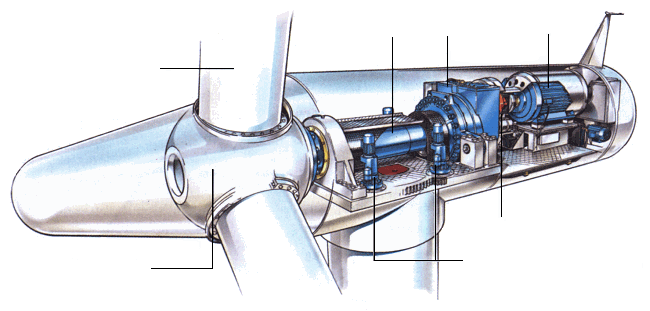
\includegraphics[width=\textwidth]{pictures/wind_turbine.png}
%	\caption{An exemplary figure}
%	\label{wind_turbine}
%	\flushleft\quad\quad\footnotesize{Source: Own illustration.}
%\end{figure}	
% ***********************************************************************************
	
% ***********************************************************************************
% Beginn des eigenstaendigen Teils
% ***********************************************************************************

\selectlanguage{english}


\chead{\textit{Introduction}}					% definiere Kopfzeile
%\include{files/Introduction}					% include statt input ermöglicht Arbeit mit \includeonly{} und fügt Seitenumbruch vor section ein

\section{Introduction}
To achieve the highly ambitious goal of the Paris Agreement to keep global temperature increase "well below 2 degrees Celsius\cite{ParisAgreement2018} " in this century, an unparalleled transformation of the energy sector is required. Germany sees itself as a leader in this effort, as one of the first countries to encourage a large scale shift of electricity generation towards renewable sources. Presently however, the country is set to miss its 2020 goals for $CO_2$ mitigation and while it is phasing out relatively $CO_2$-neutral nuclear power \cite{NuclearPowerGermany2019}, over 30 percent of electricity production still comes from coal and lignite plants, which are expected to remain running until 2035, while experts claim a coal exit by 2030 is necessary for the Paris goals to remain attainable.\cite{yanguasparraScienceBasedCoal2018}
\\
Despite this ,the continually falling costs for small scale energy generation equipment such as photovoltaics (pv) panels and fuel cells and the rising cost of electricity has spawned a new movement favouring decentralised energy generation. This trend is further propelled, by ever more affordable energy storage devices, which enable solar energy to be used throughout the night.
\\
The idea of a microgrid proposes to take the idea of decentralization a step further by creating local autonomous grids that only interact with the main grid if necessary or advantageous.
A microgrid in literature is defined as a small geographically bounded zone with clear electrical boundaries, that manages local loads and possibly contains generation units and storage. Furthermore it can be connected to the egrid, from whose perspective it is seen as a single entity. \\
Proponents of the idea promise a more inclusive and resilient power supply with no single points of failure. Furthermore the electricity grid needed to balance the few loads the microgrids cannot manage themselves would be a lot less expensive in investment and maintenance, and the consumption of locally produced electricity would lead to far less transmission losses.
\\
Critics however, point out that microgrid infrastructure and especially the needed generation and storage units are expensive, while centralized generation and transmission infrastructure already exists. They argue that, even if microgrid operators are able to be profitable, it is by avoiding taxes and levies on power, which make up over half of the German retail power prices \cite{Monitoringbericht20182018} and not by actually being competitive with centralized generation \cite{heindlIstEnergiewendeSozial2014}.
\\
At present the concept is tested in a few case studies such as in Brooklyn \cite{mengelkampDesigningMicrogridEnergy2018} and on several North American university campuses \cite{chenowethRiseUniversityMicrogrids2018}, but still little is known about its performance in applications ranging from residential areas to hospitals.
\\
Although there will no doubt be more pilot projects in the coming years, considering the trends outlined above, which propel this phenomenon remain unbroken, there is a demand for a more thorough and intuitive understanding of the performance of such a project under various conditions, without substantial risk involved.
\\
Mathematical models have proven a strong tool for a better understanding of many complex systems in the sciences but also in all engineering disciplines. Among them, Linear Programming has long been used to model electricity systems due to its high performance even for complex problems. Linear Programming (or Linear Optimization) is a method for solving mathematical models whose features can be expressed as linear relationships \cite{goodarziLinearOptimization2014}. The solution space is a convex polytope, which makes finding the optimal solution a lot faster, since there cannot be any local maximum, which is not also a global maximum. As subcategory of LP is Mixed Integer Linear Programming (MILP), which in addition to the linear relationships and variables used in LP, introduces variables which can only take integer values. While slower, it can find an optimal solution reasonably quick by using the solution of the corresponding linear problem and applying the branch- and bound algorithm \cite{MixedIntegerProgrammingMIP2018}. 
\\\\
In this thesis my aim is to develop a flexible modeling tool suitable for optimizing a microgrid setup under diverse conditions. In addition to modeling any kind of small scale generation or storage unit, the modeling tool should be able to reflect trade between connected entities as well as behaviour such as load shifting and curtailment. The objective of the model will be to meet the demand of all connected entities at a minimum cost. In addition to these functionalities at a small solving time, the modeling tool should meet the criteria of being scalable, flexible in regard to the form and quality of input data and as user-friendly as possible.\\
To demonstrate the modelling tools performance, a case study will be conducted for a small community in the German state of Northrine-Westphalia, where the majority of the German lignite capacity is located. The robustness of the results will be confirmed through a sensitivity analysis.
I expect the case study to show wether such a system is currently commercially viable in Northrine-Westphalia and, to a lesser extent, if decentralised energy management in the form of microgrids is competitive compared to the prevailing centralised solution.
All code written, as well as all other documents, including this one, will be published on github.com \cite{MITLicense2018} under an MIT license.
\\
In the following chapters a literature review will be conducted to reflect the current state of microgrid research. Then the model constructed will be described in mathematical terms, followed by a brief overview of the technical implementation. Finally, a case study including a sensitivity analysis is conducted, before conclusions are drawn from its result.

\newpage
\chead{\textit{Literature Review}}	

\section{Literature Review}
In this section I shall attempt to give an overview over the current status quo regarding the optimizaton of microgrids and more especially the tools available to do so. I will pursue  this by answering a number of broad question, which I think are crucial regarding my subject. The procedure will be structured by utilizing a consistent and reproducible methodology described in detail below. In addition to scientific literature other sources will also be taken into account at my discrection if they are neccessary or helpful in answering a question.

\subsection{Key Questions}
This literature review will attempt to answer the following key questions in the context of my subject:
\begin{enumerate}
	\item What are the most eminent scientific standards for modelling a microgrid allocation and dispatch?
	\item What is usually within the scope of such a model (what types of generation assets, only electricity or also thermal energy and so on)? 
	\item What are the common methods used to determine some of the key variables required in such a model such as interest rates, CAPEX and OPEX of assets and so on?
	\item What are the most commonly used (commercial) tools for optimizing a microgrid? Are there any free or open source solutions? 
\end{enumerate} 

\subsection{Methodology}
To arrive at a dataset of scientific literature that is reproducible I use the methodology described in \cite{petersenSystematicMappingStudies} and \cite{pop00975}:

\begin{enumerate}
	\item Define a search string
	\item Choose scientific databases to which to apply that search string
	\item Due to the possibly large amount of papers brought up by this kind of search I am only considering the 100 most relevant papers from each database.
	\item Define keywords, which have to occur in the abstracts of the publications. All publications that lack a keyword are discarded.
	\item Define Inclusion as well as Exclusion criteria. A publication must satisfy all inclusion criteria as well as none of the exclusion criteria to be included in the literature review.
\end{enumerate}
Due to the nature of some of the questions I am trying to answer in my literature review it is additionally necessary to include further non-scientific sources as well as additional scientific sources at my discretion.
The search strings, used databases, as well as the result at each step is be included in the appendix.

\subsection{Descriptive Analysis}
After filtering the original dataset of 275 unique publications in the way described in the last chapter, I arrive at a set of 61 publications. The publication year, as can be observed in Figure 1 is for most publications quite recently: 27 out of 61 papers were published 2017 and after. This could indicate a rising interest in the subject, but is probably at least partly due to the way the different search engines employed compute relevancy.  
\begin{figure}[H]
	\centering
	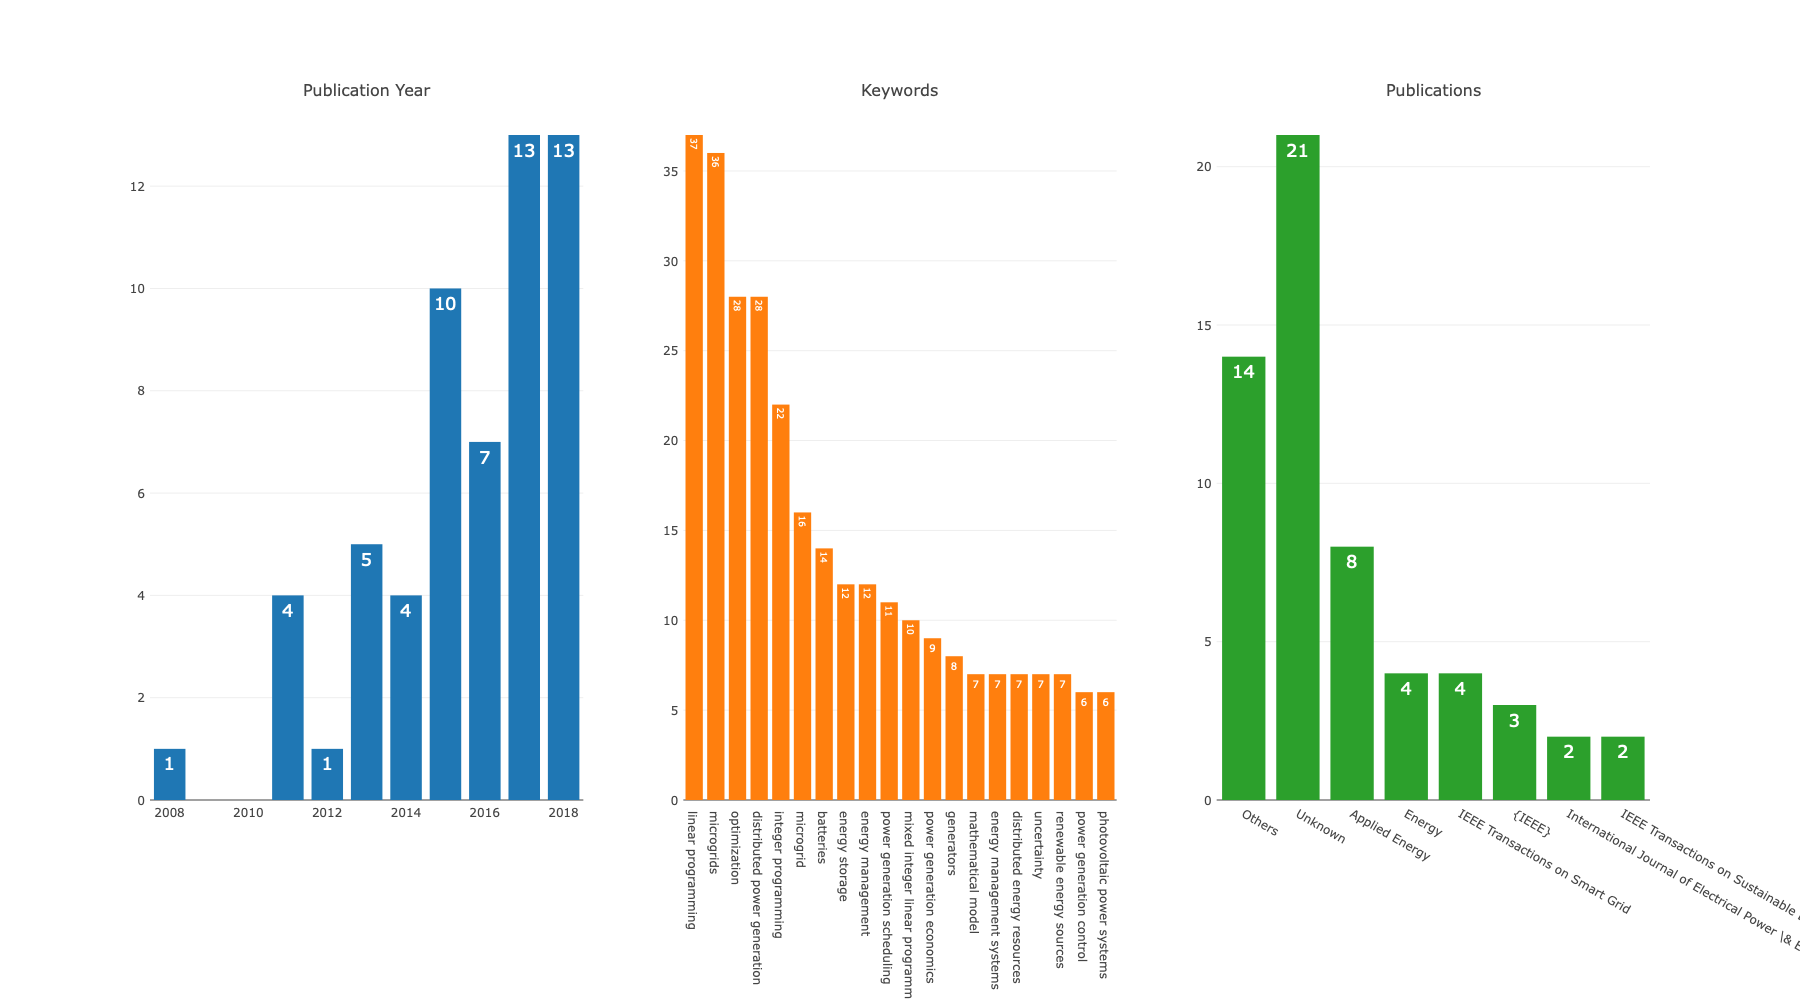
\includegraphics[width=\textwidth]{pictures/Figure_1.png}
	\caption{Results of an automated descriptive analysis}
	\label{descriptive_anaylsis_results}
	\flushleft\quad\quad\footnotesize{Source: Own illustration.}
\end{figure}	
Looking at the keywords used to describe the publication shows that, unsurprisingly, the most often occuring keywords are the ones used in conducting the search: 'linear programming', 'microgrids' and 'optimization'. 'distributed energy generation' and 'distributed energy resources'are mentioned 37 times, 'batteries' and 'energy storage' a total of 28 times, and 'renewable energy sources' and 'generators' a total of 16 times. This illustrates the focus on decentralized energy sources and storage, more specifically renewables and small scale combined heat and power generation that prevails throughout the literature.
\\
The publication chart is not very enlightening. This is due to the fact 28 out of 61 publications are conference papers which either appear under others because there is only one instance of that particular conference or unknown. From a more general point of view though almost all papers are published either by Elsevier or IEEE, with very few exceptions.


\subsection{Literature Overview}
The first question in need of an answer in optimizing a microgrids design and dispatch is the question of the modelling approach itself. Although the dataset of literature derived from the methodology described in 2.2 is biased towards Linear Programming, which was one of the search and filter criteria, it contains multiple employed methodologies. For example, \cite{7975049} employ both a Mixed Integer Linear Programming (MILP) model and a Genetic Algorithm (GA) and come to the conclusion that while both deliver accurate and robust results the MILP model is faster. \cite{NEMATI2018944} mostly concur. While in this case, the results of the GA were better in two scenarios, it was outperformed by the MILP model in the remaining three.
A key problem of MILP however seems to be its deterministic nature, which anticipates perfect knowledge of all the parameters involved. Especially for optimisation problems regarding a short timeframe, such as day-ahead scheduling this is a significant problem, since actual parameters may be different. Several methods addressing this problem can be found in literature. 
\\
One such method are rolling time horizons. This approach optimizes the dispatch of a microgrid for a fixed time horizon based on steadily updated forecasts of the uncertain paremeters. The optimization is repeated periodically to reflect the updated forecasts \cite{palma2013microgrid} \cite{silvente2015rolling} and increase dispatch accuracy in the nearer future. Rolling Horizon Optimization is however unfit to optimize investment, since it is not possible to adapt investment decisions ex post to changed conditions.
\\
While the rolling time horizon method helps to limit uncertainty by reacting to changes of input parameters, Robust Optimization and Stochatsic Optimization try to proactively account for a variety of possible scenarios. Robust Optimization achieves this by optimizing for a number of scenarios deemed equally likely, as in \cite{CRAPARO2017135} using ensemble weather forecasts or in \cite{8240914} and \cite{zhang2015optimal} using upper and lower boundaries for uncertain parameters. Stochastic Optimization on the other hand uses detailed probability distributions to weigh the probability of each scenario occuring as explained in \cite{7540870}. To arrive at these distributions secondary tools are usually needed. Shams et al use a simple Gaussian randomization to make their demand data reflect uncertainty, as well as more specific distributions for irridiation and wind speeds. A number of other methodologies appear in literature such as employing a Monte Carlo simulation \cite{ZHENG2018204} or deriving multiple scenarios and corresponding realization probabilities from historical data \cite{7244857}.
\\
The scope of the microgrid models found in literature varies greatly. A constant however is the definition of a microgrid as bounded, operating in a small geographical zone and with a clear electrical boundaries \cite{TAVAKOLI20181}\cite{mashayekhMixedIntegerLinear2017}\cite{7853085}; managing local loads \cite{zhang2013efficient} \cite{ZHENG2018836}; possibly containing various generation units and storage \cite{silvente2015rolling}\cite{7741704} and possibly being able to exchange power with the main grid \cite{NEMATI2018944}\cite{SOLTANINEJADFARSANGI2018257}, from whose perspective it is seen as a single entity \cite{KOLTSAKLIS2018318}.
\\
While most of the selected literature consider cases where a grid connection exists and can be used at all times, there is a number of publications that consider either completely islanded microgrids \cite{ZHANG20181229}\cite{palma2013microgrid} \cite{6872087}\cite{7281564} or microgrids that can sustain themselves in islanded mode for extended periods for exapmle in case of natural disasters \cite{TAVAKOLI20181}.
\\
The clearest distinctions between microgrid models, after the object and applied methodology is properly defined, is based on the aspect or aspects that the model is supposed to optimize. The literature can be split in two groups, either optimizing only dispatch or both investment (e.g. the planning phase) and dispatch. The former group is definitely the larger, with only 12 out of 61 publications considering investment. Notably only one of these \cite{7540870} uses any of the methods to model uncertainty discussed above.
\\
There is also significant diversity in literature when it comes to the technologies considered in modelling.
Modelling dispatchable (eg. non-renewable) as well as non-dispatchable (eg. renewable) generation is rather common, but the specifics differ:
While most models consider PV or Wind as well as a CHP generator, the included generation technologies are as diverse as geothermal generators \cite{7975049} and gas turbines \cite{UMEOZOR2016272} \cite{NEMATI2018944}. In addition to modelling electricity, some publications also consider heat generation and transmission \cite{LAUINGER201624}\cite{wouters2015energy}. This is valuable, because the economic performance of a non-renewable generation unit (usually CHP) present in most models depends heavily on if and how the heat is used, as \cite{costa2014mixed} point out.
\\
The types of storage used in literature also vary. Although battery storage \cite{7399422}\cite{UMEOZOR2016272}\cite{6465822} or an abstract storage device \cite{6669807}\cite{zhang2011optimal} are the most common choices, there are a number of papers modeling heat storage \cite{zhang2013efficient}\cite{zhang2015optimal}\cite{LAUINGER201624}\cite{wouters2015energy}, and some with more exotic technology choices such as flywheels \cite{6700453} or an electrolyzer \cite{7125149}.
\\
In addition to these generation and storage technologies some publications also model the network topology \cite{8023785}\cite{7972908}\cite{SHAMS2018326} and some even consider electrical phenomena such as active and reactive power losses \cite{7741704}\cite{mashayekhMixedIntegerLinear2017} and voltage deviation \cite{7741704}. 
\\
Demand side management, which some models implement is usually represented by dividing loads into different categories. \cite{7972908} distinguish between 'critical loads' ,meaning loads that absolutely have to be satisfied, 'shiftable loads', meaning loads that have to be satisfied, although there is a time window, rather than an exact point in which they can be serviced, and 'adjustable' loads, which can be dropped if needed. Although the terms may vary, and many publications do not introduce the 'shiftable loads' category alltogether, these conceptual distinctions are made by a number of other authors \cite{silvente2015rolling}\cite{zhang2015optimal}\cite{8216436}.
\\
The model results depend almost as much on the given input parameters used in case studies as on the modelling approach itself. There is however only a limited number of publications with detailed documentation of the parameters used.
The used parameters can be broadly categorized as either economic parameters, such as capital and operation and maintenance cost for the technologies used, generation related parameters such as irradiation and wind speeds, and load data, representing consumer behaviour.
\\
In publications documenting cost parameters there is a clear trend towards a split of technology cost into investment and maintenance cost. However, whereas \cite{LAUINGER201624} define maintenance cost as a fixed cost per unit of time, \cite{wouters2015energy} define it as a function of kilowatthours produced, a measurement which \cite{LAUINGER201624} call 'fuel costs'. \cite{7399422} choose a definition closer aligned with the former, they however define yearly maintenance cost simply as a flat percentage of the units' investment cost.\cite{KOLTSAKLIS2018318} seem to neglect maintenance costs alltogether focusing only on investment costs. While some models document econimic paramters such as discount rates \cite{7399422}, many don't and it is unclear if future flows of value are properly discounted in these models. Furthermore many of the publications declare cost parameters as assumptions rather than trying to derive them from sources, although a few such as \cite{LAUINGER201624} and \cite{wouters2015energy} do so.
\\
The selected literature offers multiple ways of obtaining input parameters of metereological data. \cite{7981571} use historical metereological data while \cite{palma2013microgrid} build a prediction model for forecasting irridiation and wind speeds. Similarly there are authors who use historical data for load parameters such as \cite{7981571} and ones who generate synthetic data based on appliance use and probabilistic models \cite{zhang2013efficient}\cite{zhang2011optimal}\cite{zhang2015optimal} or neural networks using empirical data \cite{palma2013microgrid}.
\\
When it comes to modelling tools DER-CAM \cite{LAUINGER201624}\cite{ZHENG2018204}\cite{8023785} and HOMER \cite{amrollahi2017techno}\cite{ZHENG2018204}\cite{LAUINGER201624} are the most often referenced. DER-CAM or Distributed Energy Resources Customer Adoption Model is an optimizatioon tool developed at Berkeley Labs and uses Mixed Integer Linear Programming to optimize portfolio, placement, sizing and dispatch of Microgrid Energy Systems \cite{DistributedEnergyResources2018}. HOMER Grid is a commercial optimization tool for behind the meter systems. Its main advantage is it's large database of components and tariff rates in the United States and Canada \cite{HOMERGridBehindtheMeter2018}. The most often mentioned solver is the CPLEX commercial solver \cite{sechilariu2014supervision}\cite{NEMATI2018944}\cite{UMEOZOR2016672}\cite{7741704}... . Most of the models are written in GAMS \cite{silvente2015rolling}\cite{UMEOZOR2016672}\cite{CRAPARO2017135}..., although many are written in MATLAB \cite{7741704}\cite{7972908}... .
\\
Open source tools seem scarcely available. A search of 'microgrid optimization' on github.com, the major open source software platform, brings up only 3 items with more than one star, none of them has more than ten (popular libraries might have thousands)\cite{GithubSearchMicrogrid2018}. The most up-to-date one has not been updated for a year and none features a graphical user interface.

\newpage
\chead{\textit{Mathematical Formulation}}	
\section{Mathematical Formulation}
\todo{references for all equations}
\todo{all parameters, variables table}
\subsection{Time}
The range of scenarios and complexity the model can handle is, among other things, dependant on its implementation of discrete time. More and smaller timesteps and a representative sample of diverse expectable conditions regarding the parameters leads to higher model accuracy. Of course the amount of timesteps is limited by processing power and therefore by model complexity. To enable both diverse and therefore potentially discontinuous parameter sets and a reasonable length for each set, the length of 1 hour is chosen for the basic timestep 
$t; t \in [1,T]; T \in \mathbb{N} ;$. $T$ denotes the number of hours in each discontinuous sets of supply and demand parameters.
Furthermore the ability of including multiple discontinuous sets of supply and demand parameters of the same length in one scenario is gained by introducing a second iterator 
$s; s \in [1,S]; S \in \mathbb{N} ;$. $S$ denotes the number of discontinuous sets of supply and demand parameters.





\subsection{Households}
To properly conduct trading and for the future possibility of adding voltage and topological constraints to the model, the households are modelled as independent entities, each with its own demand, generation and storage. Therefore a third iterator $u; u \in [1,U]; U \in \mathbb{N};$ is introduced. $U$ denotes the number of households modelled.
An abstract household $H$ is defined as a tuple of storage and generation devices as well as demand curves. For discrete storage and generation devices two separate sets of positive integers define how much of each option available in the scenario was installed. Additionally each household has a price $shiftP$ and $curtP$ at which they are willing to shift or curtail a unit  of their load respectively.
\begin{equation}
	H := (GEN, ST, dGEN, dST, DEM, shiftP, curtP)
\end{equation}

A concrete household $H_u$ implements these values:
\begin{equation}
	GEN \in \mathbb{R}^{K}; GEN_k \geq 0 \forall k; k\in [0,K]
\end{equation}
\begin{equation}
	ST \in \mathbb{R}^{L}; ST_l \geq 0 \forall l; l\in [0,L] 
\end{equation}
\begin{equation}
	dGEN \in \mathbb{N}^{M}
\end{equation}
\begin{equation}
	dST \in \mathbb{N}^{N}
\end{equation}
with\\
$k,l\ in \mathbb{N}$\\
and\\
$K,L,M,N \in \mathbb{N}$\\
and\\
$shiftP, curtP \geq 0$

$K$ and $L$ denote the amount of generation and storage devices in household $H_u$.This, in practice, is equal to the amount of linear scaling investment options for each category, since a zero capacity device is still modelled as a device. $M$ and $N$ denote the amount of discrete investment options in their respective category. $GEN_k$ and $ST_l$ are the capacities installed of the k-th and l-th linear investment option respectively. $GEN_m$ and $dST_n$ are the amount installed of the m-th and n-th discrete investment option available. $DEM$ is further defined in the subsection demand.
\\
A list of instances of the structure $H$ and its length $U$ are both model parameters.





\subsection{Internal Variables}
The objective of the model is to find optimal investment, dispatch and trade. Therefore, the following sets of internal parameters are introduced:
	\\
	$\forall u,s,t$:
	\begin{equation}
		toTR_{u,s,t}, fromTR_{u,s,t} \geq 0
	\end{equation}
	The trade supply variables $toTR_{u,s,t}$ and $fromTR_{u,s,t}$ reflect the amount of traded power, to the trading pool and from the trading pool, respectively. They are defined for each household at each timestep.
	\\\\
	$\forall u,k,m,s,t$:
	\begin{equation}
		genS_{u,k,s,t}, dgenS_{u,m,s,t} \geq 0
	\end{equation}
	The generation supply variables $genS_{u,k,s,t}$ and $dgenS_{u,m,s,t}$ describe the amount of energy produced by each linear or discrete generation option respectively. They are defined for each generation option in each household and at each timestep. It is useful to keep in mind though, that not every household needs to implement all the generation options. In case of zero instances of the discrete generation option $dGEN_2$ installed in household $H_5$, for example, $dgenS_{5,2,s,t} = 0$ for all $s$ and $t$.
	\\\\
	$\forall u,l,n,s,t$:
	\begin{equation}
	fromST_{u,l,s,t}, toST_{u,l,s,t}, fromDST_{u,n,s,t}, toDST_{u,n,s,t} \geq 0
	\end{equation}
	The storage supply variables $fromST_{u,l,s,t}$ and $toST_{u,l,s,t}$ indicate the amount of power fed into or withdrawn from a linear storage investment option. They are defined for each linear investment option and each household at each timestep. The variables $fromDST_{u,n,s,t}$ and $toDST_{u,n,s,t}$ have the equivalent function for all discrete storage investment options.	
	\\\\
	$\forall u,s,t$:
	\begin{equation}
		toSC_{u,s,t}, fromSC_{u,s,t} ncS_{u,s,t},  \geq 0
	\end{equation}
	The shifted consumption supply variable $toSC_{u,s,t}$ represents the amount of power consumtion shifted by each household at each timestep.  $fromSC_{u,s,t}$ indicates the amount of power consumption that has previously been shifted and is now consumed. The non-consumption supply variable $ncS_{u,s,t}$ designates the amount of power consumption curtailed for each household at each timestep.
	\\\\
	$\forall u,s,t$:
	\begin{equation}
		fromGR_{u,s,t}, toGR_{u,s,t} \geq 0
	\end{equation}
	Finally, the grid supply variables $fromGR_{u,s,t}$ and $toGR_{u,s,t}$ denote the amount of power supplied by and to the respectively by each household at each timestep. Only power flowing out of and into the microgrid included in this definition, power traded internally, while using the (micro)grid, is reflected in the trade variables. (see formula (6))
	
	$\forall u,k$:
	\begin{equation}
		H_u\hookrightarrow GEN_k \geq 0
	\end{equation}
	$\forall u,l$:
	\begin{equation}
		H_u\hookrightarrow  ST_l \geq 0
	\end{equation}
	$\forall u,m$
	\begin{equation}
		H_u\hookrightarrow d GEN_m \in \mathbb{N}
	\end{equation}
	$\forall u,n$
	\begin{equation}
		H_u\hookrightarrow d ST_n \in \mathbb{N}
	\end{equation}
	$H_u\hookrightarrow GEN_k$, $H_u\hookrightarrow  ST_l \geq 0$, $H_u\hookrightarrow d GEN_m$, $H_u\hookrightarrow d ST_n$ are variables describing the realized capacities of each linear and discrete investment option in each household. They are explained in more detail in section 3.2.





\subsection{Generation}
For a model, explicitly built to optimize decentralized generation in microgrids, a robust and flexible mathematical representation of generation options is required.
Therefore an abstract linear generation device $GEN$ and an abstract discrete generation device $dGEN$, which can represent a range of technology options, are defined:\\
	\begin{equation}
		GEN := (C_{Cap}, C_{OpFix}, C_{OpVar}, T_{Life}, EFF_{el}, PR, maxFl)
	\end{equation}
	\begin{equation}
		dGEN := (CAP, C_{Cap}, C_{OpFix}, C_{OpVar}, T_{Life}, EFF_{el}, PR, maxFl)
	\end{equation}
	$CAP \geq 0$, which is only required for discrete investments, defines the generation capacity of the discrete investment option.
	$C_{Cap} \geq 0$ defines the total investment cost for discrete generation devices. For linear generation devices the investment cost is expressed in terms of one unit of capacity.
	$C_{OpFix} \geq 0$ expresses the fixed maintenance cost per unit of time. In the case of linear generation they expressed in proportion to capacity, while for discrete generation they express the maintenance cost of one discrete device.
	$C_{OpVar} \geq 0$ expresses the variable maintenance cost per unit of input consumed.
	$T_{Life} \in \mathbb{N}$ defines the life expectancy of a generation device, e.g the time before it is replaced. 
	$EFF_{el} \in [0,1]$ defines the ratio of supplied energy, for example sunlight or gas, to produced electricity.
	$PR \in [0,1]$ is another definable penalty to electricity production, which can, for example, express the degradation of solar cells. 	
	$maxFl \in \mathbb{R}^{S \times T}, maxFL \geq 0 \forall s,t$ denotes the maximal possible flow of input energy, e.g. sunlight in case of solar pv or gas in case of a fuel cell. This enables the represantation of intermittent availability for wind and solar. It could nevertheless be used to model any condition that would restrict a conventional generation device from running at capacity at certain times, for example air quality regulation.  \\
	All instances of the $GEN$ structure are collected in one list. The same is true for all instances of the $dGEN$ structure. These lists and their sizes $K$ and $M$ are parameters. The model uses the iterators $k$ and $m$ to represent individual instances of these structures. (see section 3.2)
	\\
	In addition, to model generation appropriately, several sets of constraints need to be defined:
	
	$\forall u,k,s,t$:
	\begin{equation}
		\begin{split}
		genS_{u,k,s,t} \leq min(\frac{GEN_k \hookrightarrow EFF_{el} * GEN_k \hookrightarrow maxFl_{s,t}}{H_u\hookrightarrow  GEN_k}, 1) \\ * H_u\hookrightarrow  GEN_k * GEN_k \hookrightarrow PR
		\end{split}
	\end{equation}
	\\
	$\forall u,m,s,t$:
	\begin{equation}
		\begin{split}
		dgenS_{u,m,s,t} \leq min(\frac{GEN_m \hookrightarrow EFF_{el} * GEN_m \hookrightarrow maxFl_{s,t}}{H_u \hookrightarrow  dGEN_m * dGEN_m \hookrightarrow CAP }, 1) \\ * H_u\hookrightarrow  dGEN_m * dGEN_m \hookrightarrow CAP * dGEN_k \hookrightarrow PR
		\end{split}
	\end{equation}
	The capacity constraints restrict the use of any linear generation device $GEN_k$ or any discrete generation device $dGEN_m$ to its capacity rating and the maximum flow of input energy supplied to it.
	The constraints differ due to the capacity of linear generaton devices being stored in the household structure directly, while for discrete generation devices the household structure only contains an integer representing the amount implemented. This value is then multiplied with the capacity of one unit of the concerned discrete generation device to compute the total installed capacity. In both cases the result is multiplied with the performance ratio $PR$ of the concerned device, which acts as a penalty to capacity(see above). The minimized term calculates the ratio of maximum output achievable with the available maximum input to the capacity of the device. If the input suffices for running at capacity the term returns a maximum of 1, not restricting supply further, otherwise it restricts capacity to the maximum possible under current resource input.

	






\subsection{Storage}
The introduction of the concept of energy storage is necessary if the use of a large proportion of intermittent power production while maintaining intermittent power demand is to be seriously explored.
Therefore an abstract linear storage device $ST$ and an abstract discrete storage device $dST$, which can represent a range of technology options, are defined:\\
	\begin{equation}
		ST := (C_{Cap}, T_{Life}, EFF_{+-}, maxP_{+}, maxP_{-})
	\end{equation}
	\begin{equation}
		dST := (CAP, C_{Cap}, T_{Life}, EFF_{+-}, maxP_{+}, maxP_{-})
	\end{equation}
	$CAP \geq 0$, which is only required for discrete investments, defines the usable capacity of the discrete investment option.
	$C_{Cap} \geq 0$ defines the total investment cost for discrete storage devices. For linear storage investment options the investment cost is expressed in terms of one unit of capacity.
	$T_{Life} \in \mathbb{N}$ defines the life expectancy of a storage device, e.g the time before it is replaced. To be able to better estimate this value it is assumed, that storage is, on average, cycled once per day.
	$EFF_{+-} \in [0,1]$ defines the roundtrip efficiency, e.g. what proportion of one unit of power is left after charging and discharching inefficiencies. It is used to compute the charge and discharge efficiencies.
	The charge efficiency $EFF_{+}$ is defined as $EFF_{+} = \sqrt{EFF_{+-}}$ and the discharge efficiency $EFF_{-}$ as $EFF_{-} = 1/EFF_{+}$.\cite{LAUINGER201624}\\
	$maxP_{+} \geq 0$ and $maxP_{-} \in [0,1] 0$ denote the maximum charge rate and discharge rate respectively, relative to the devices capacity.
	All instances of the $ST$ structure are collected in one list. The same applies for all instances of $dST$. The two lists and their sizes $L$ and $N$ are model parameters. The model uses the iterators $l$ and $n$ to represent individual instances of these structures. (see section 3.2)
	\\
	To model storage appropriately several sets of constraints need to be specified:
	\\
	$\forall u,l,s,t $:
	\begin{equation}
		toST_{u,l,s,t} \leq ST_l\hookrightarrow  maxP_{+} * H_u \hookrightarrow ST_l
	\end{equation}
	\begin{equation}
		fromST_{u,l,s,t} \leq ST_l\hookrightarrow  maxP_{-} * H_u \hookrightarrow ST_l
	\end{equation}
	\\
	The flow constraints for linear storage constrain the maximum in- and outflow for each linear storage device to its maximum in- and outflow rate relative to capacity.
	\\
	$\forall u,n,s,t$:
	\begin{equation}
		toDST_{u,n,s,t} \leq dST_n\hookrightarrow  maxP_{+} * H_u \hookrightarrow dST_n * dST_n \hookrightarrow CAP
	\end{equation}
	\begin{equation}
		fromDST_{u,n,s,t} \leq dST_n\hookrightarrow  maxP_{-} * H_u \hookrightarrow dST_n * dST_n \hookrightarrow CAP
	\end{equation}
	The flow constraints for discrete storage work similar to the linear ones, with the slight distinction of how capacity is computed. Rather than stored directly in the $H_u$ structure, it is stored as an attribute of the discrete storage device structure $dST_n$ and is multiplied by the integer amount of units implemented stored in $H_u$. (see 3.2)
	\\
	$\forall u,l,s$:
	\begin{equation}
		\sum_{t=1}^{T}(ST_l \hookrightarrow EFF_{+} * toST_{u,l,s,t'} - ST_l \hookrightarrow EFF_{-} * fromST_{u,l,s,t'}) = 0
	\end{equation}
	\\
	$\forall u,n,s$:
	\begin{equation}
		\sum_{t=1}^{T}(dST_n \hookrightarrow EFF_{+} * toDST_{u,n,s,t'} - dST_n \hookrightarrow EFF_{-} * fromDST_{u,n,s,t'}) = 0
	\end{equation}
	\\
	The model assumes the storage to be full at the start of each simulated discontinous period $s$ and requires it to be full at the end of each period. This means inflows minus outflows weighted by the respective efficiencies need to sum up to zero for the entirety of each period $s$.
	\\
	$\forall u,l,s,t$:
	\begin{equation}
		\begin{split}
		toST_{u,l,s,t} * ST_l \hookrightarrow EFF_{+} \leq \\
		\sum_{t'=1}^{t-1}(-ST_l \hookrightarrow EFF_{+} * toST_{u,l,s,t'} + ST_l \hookrightarrow EFF_{-} * fromST_{u,l,s,t'})
		\end{split}
	\end{equation}
	\\
	$\forall u,n,s,t$:
	\begin{equation}
		\begin{split}
		toDST_{u,n,s,t} * dST_n \hookrightarrow EFF_{+} \leq \\
		\sum_{t'=1}^{t-1}(dST_n \hookrightarrow EFF_{+} * toDST_{u,n,s,t'} - dST_n \hookrightarrow EFF_{-} * fromDST_{u,n,s,t'})
		\end{split}
	\end{equation}
	\\
	The storage capacity constriants prohibit storage usage beyond the storage devices capacity. The remaining storage capacity at time $(s,t)$ is in theory calculated as the capacity minus current storage level, which is the sum of all inflows and outflows weighted by in- and outflow efficiency. Since the storage at each timestep $(s,0)$ is required to be full, the capacity is subtracted once, which eliminates it and leaves only the sum. The constraint is implemented equivalently for discrete storage. 
	\\
	$\forall u,l,s,t$:
	\begin{equation}
	\begin{split}
		fromST_{u,l,s,t} * ST_l \hookrightarrow EFF_{-} \leq H_u \hookrightarrow ST_l +\\
		\sum_{t'=1}^{t-1}(ST_l \hookrightarrow EFF_{+} * toST_{u,l,s,t'} - ST_l \hookrightarrow EFF_{-} * fromST_{u,l,s,t'})
		\end{split}
	\end{equation}
	\\
	$\forall u,n,s,t$:
	\begin{equation}
	\begin{split}
		fromDST_{u,n,s,t} * dST_n \hookrightarrow EFF_{-} \leq H_u \hookrightarrow dST_n * dST_n \hookrightarrow CAP +  \\
		\sum_{t'=1}^{t-1}(dST_n \hookrightarrow EFF_{+} * toDST_{u,n,s,t'} - dST_n \hookrightarrow EFF_{-} * fromDST_{u,n,s,t'})
	\end{split}
	\end{equation}
	Finally, the storage level constraints prohibit the storage level to fall below zero. This means there can be no more power withdrawn, weighted by outflow efficiency, than is currently stored in the device. Because we assume the storage to be full at the start of each period $s$, the current charge amounts to one full charge (storage capacity) plus the sum of all transactions during the current period up to the current timestep $t$. The only distinction for discrete storage devices is the way capacity is calculated. (see 3.2)




\subsection{Trade}
Trade is implemented as an exchange platform, which sums up deposits and withdrawals of power at each timestep and always needs to be balanced. This approach has the advantage of reducing the number of constraints and therefore complexity greatly, although it is not very well suited to handle grid topology constraints which might be added in the future.\\
The trade constraint is defined as:
\\

$\forall s,t$:
\begin{equation}
	\sum_{u = 1}^{U}(toTR_{u,s,t}-fromTR_{u,s,t}) = 0
\end{equation}





\subsection{Demand}
Abstract demand data $DEM$ is defined as a set of the size $S$ of demand profile sets of the size $T$:
\begin{equation}
 DEM:= \{DEM_s | s \in [1,S]; s\in \mathbb{N}; \forall DEM_s, DEM_s := \{DEM_{s,t} | t\in [0,T]; t \in \mathbb{N}\}
\end{equation}

As frequently applied in literature, $DEM_{s,t}$ is not a demand value, but rather a tuple of three demand values, critical demand, shiftable demand and curtailable demand \cite{silvente2015rolling}\cite{zhang2015optimal}\cite{8216436}\cite{7972908} : \\
\begin{equation}
 DEM_{s,t}:= (critDEM_{s,t}, shiftDEM_{s,t}, curtDEM_{s,t}) 
\end{equation}

$\forall u,s,t$:\\
$H_u \hookrightarrow critDEM_{s,t}, H_u \hookrightarrow shiftDEM_{s,t}, H_u \hookrightarrow curtDEM{s,t} \geq 0$

Critical demand will be met by the model as it is seen as a constraint. Shiftable demand can be shifted by one hour at a fixed rate defined for each household. Curtailable demand can be dropped at a fixed rate defined for each household.
The restrictions on shiftable and curtailable demand is expressed by the following sets of contraints:
\\
$\forall u,s,t$:
\begin{equation}
	scS_{u,s,t} \leq H_u \hookrightarrow shiftDEM_{s,t}
\end{equation}
\begin{equation}
	ncS_{u,s,t} \leq H_u \hookrightarrow curtDEM_{s,t}
\end{equation}





\subsection{Grid}
The modelled microgrid is connected to the grid via a common point of coupling. The grid is defined as:
\begin{equation}
	GRID:= (maxS, maxD, gridC, feedC)
\end{equation}
with\\
$maxS,maxD, gridC, feedC \in \mathbb{R}^{S \times T}$\\
and $\forall s,t$: \\
$maxS_{s,t}, max_{s,t}, gridC_{s,t}, feedC_{s,t} \geq 0$

$maxS$ describes the maximum amount of power supplied by the grid at each timestep $(s,t)$, while $gridC_{s,t}$ expresses the price at which this power can be bought.
$maxD$ describes the maximum amount power that can be fed into the the grid at timestep $(s,t)$, while $feedC_{s,t}$ expresses the price at which the grid buys this power. 

To model the expected behaviour of the grid several sets of constraints need to be introduced:
\\
$\forall s,t$:
\begin{equation}
	\sum_{u=1}^{U}(fromGR_{u,s,t}-toGR_{u,s,t}) \leq maxS{s,t}
\end{equation}
The first grid contraint, restricts the sum of each housholds "trade balance" with the grid to the maximum power the grid can supply at each timestep.
\\
$\forall s,t$
\begin{equation}
	\sum_{u=1}^{U}(toGR_{u,s,t}-fromGR_{u,s,t}) \leq maxD{s,t}
\end{equation}
The second grid constraint does the reverse, in that it restricts the sum of each housholds "trade balance" with the grid to the maximum power the microgrid can feed into the grid at each timestep.

\subsection{Power Balance}
The power balance constraints describe the need for a balance between supply and demand at each node at each timestep: 
\\
$\forall u,s,t$:
\begin{equation}
	\begin{split}
		H_u\hookrightarrow  critDEM_{s,t} + H_u\hookrightarrow  shiftDEM_{s,t} + H_u\hookrightarrow  curtDEM_{s,t}\\
		= \\
		fromGR_{u,s,t} - toGR_{u,s,t} + \sum_{k=1}^K{genS_{u,k,s,t}} + \sum_{m=1}^M{dgenS_{u,m,s,t}} \\ 
		+ fromTR_{u,s,t} - toTR_{u,s,t} + scS_{u,s,t} - scS_{i,s,t-1} + ncS_{u,s,t} \\
		+ \sum_{l=1}^L{fromST_{u,l,s,t} - toST_{u,l,s,t}} + \sum_{n=1}^N{fromDST_{u,n,s,t}-toDST_{u,n,s,t}}
	\end{split}
\end{equation}
The power balance constraint requires electricity supply and demand to balanced for each household at each timestep. On the demand side the three types of demand of the concerned houshold and the current timestep are summed up. The supply side is made up of several terms: \\
$fromGR_{u,s,t} - toGR_{u,s,t}$ expresses the momentary trade balance with the grid, while $fromTR_{u,s,t} - toTR_{u,s,t}$ denotes the momentary trade balance with the microgrid's trading pool. $scS_{u,s,t} - scS_{i,s,t-1}$ is the balance of consumption shifted from the current timestep into the future and past shifted demand realized now. $ncS_{u,s,t}$ reflects loads dropped in the current timestep. Finally the power generated by all linear and dicrete generation devices is summed up, as well as the balance of storage use for all linear and discrete storage devices.




\subsection{Cost Minimization Formula}
The cost minimisation formula calculates the cost of all investment and dispatch decisions made:
\begin{equation}
	\min C_{total} = C_{Investment} + C_{Operation} + C_{Dispatch}
\end{equation}
The total cost can be broken down into investment, operation and dispatch costs. 
\begin{equation}
	\begin{split}
		C_{Investment} = \sum_{u=1}^{U}[\sum_{k=1}^K{(GEN_k\hookrightarrow  C_{Cap} * H_u\hookrightarrow  GEN_k)}\\
		+ \sum_{l=1}^L{(ST_l\hookrightarrow  C_{Cap} * H_u\hookrightarrow  ST_l)}\\
		+ \sum_{m=1}^M{(dGEN_m\hookrightarrow  C_{Cap} * H_u\hookrightarrow  dGEN_m)}\\
		+ \sum_{n=1}^N{(dST_n\hookrightarrow  C_{Cap} * H_u\hookrightarrow  dST_n)}]
	\end{split}
\end{equation}
The investment costs consist of all investment into generation and storage devices throughout the microgrid. In the context of the model this means for linear investment options the installed capacity times the costs of capital per unit of capacity and for discrete investment options the costs of capital for a single instance of a device multiplied with the number of instances installed.

\begin{equation}
	\begin{split}
		C_{Operation} = \sum_{u=1}^{U}[\sum_{k=1}^{K}(GEN_k\hookrightarrow  C_{OpFix} * H_u \hookrightarrow GEN_k * S * T)\\
	 	+ \sum_{m=1}^{M}(dGEN_m\hookrightarrow  C_{opFix} * H_u \hookrightarrow GEN_m * S * T)]
	\end{split}
\end{equation}
The operation costs are the sum of all fixed operation costs of all generation devices deployed. They are calculated for each investment option in each household by multiplying its fixed operation costs with the installed capacity (or pieces in the case of discrete investment options) and the total number of timesteps. The sum over all of these investment options are the total maintenance costs for generation in the microgrid. Since there is no fixed maintenance cost defined for storage this value is equal to all the maintenance costs incurred.

\begin{equation}
	\begin{split}
		C_{Dispatch} = \sum_{s=1}^{S}\sum_{t=1}^{T}\sum_{u=1}^{U}[gridC_{s,t} * fromGR_{u,s,t} - feedC_{s,t} * toGR_{u,s,t}\\
		+ H_u\hookrightarrow  curtP * ncS_{u,s,t} + H_u\hookrightarrow  shiftP * scS_{u,s,t}\\
		+ \sum_{k=1}^K(GEN_k\hookrightarrow  C_{OpVar} * genS_{u,k,s,t})\\ 
		+ \sum_{m=1}^M(dGEN_m\hookrightarrow  C_{OpVar} * dgenS_{u,m,s,t})]
	\end{split}
\end{equation}

The dispatch cost consist of the fuel costs (or variable operation costs $C_{OpVar}$) incurred by the use of all deployed generation devices as well as the value of all shifted and curtailed loads. In addition all transactions with the main grid are valued at the power and feed-in rates for their respective timestep and summed up.



\newpage
\chead{\textit{Technical Implementation}}	
\section{Technical Implementation}
The performance of a modeling tool depends as much on its implementation, as on mathematical soundness. In this section the choices made implementing the model described in the previous section are outlined.\\
The implementation of the modeling tool pursues multiple objectives:
\begin{itemize}
	\item Performance: The ability to solve the problem adequately fast.
	\item Scalability: The ability for the system to potentially be used by many users concurrently, without encountering performance issues.
	\item Flexibility: The ability to receive a wide range of differently formatted input data and still function adequately. Sparse, or otherwise lacking input data is preprocessed, and can be supplemented by default values.
	\item User-Friendliness: The tool offers a user-friendly way of inputting data and of viewing computation results, possibly through a graphical interface.
\end{itemize}
\subsection{Architecture}
To address these objectives the modeling tool was designed to work as a multi-layer architecture, with each layer performing a distinct part of the work flow. It is important to note however, that, while these layers can run on seperate machines to provide scalability, they do not have to. In the setup used for conducting the case study all layers were run on a single machine. 
\begin{figure}[H]
	\centering
	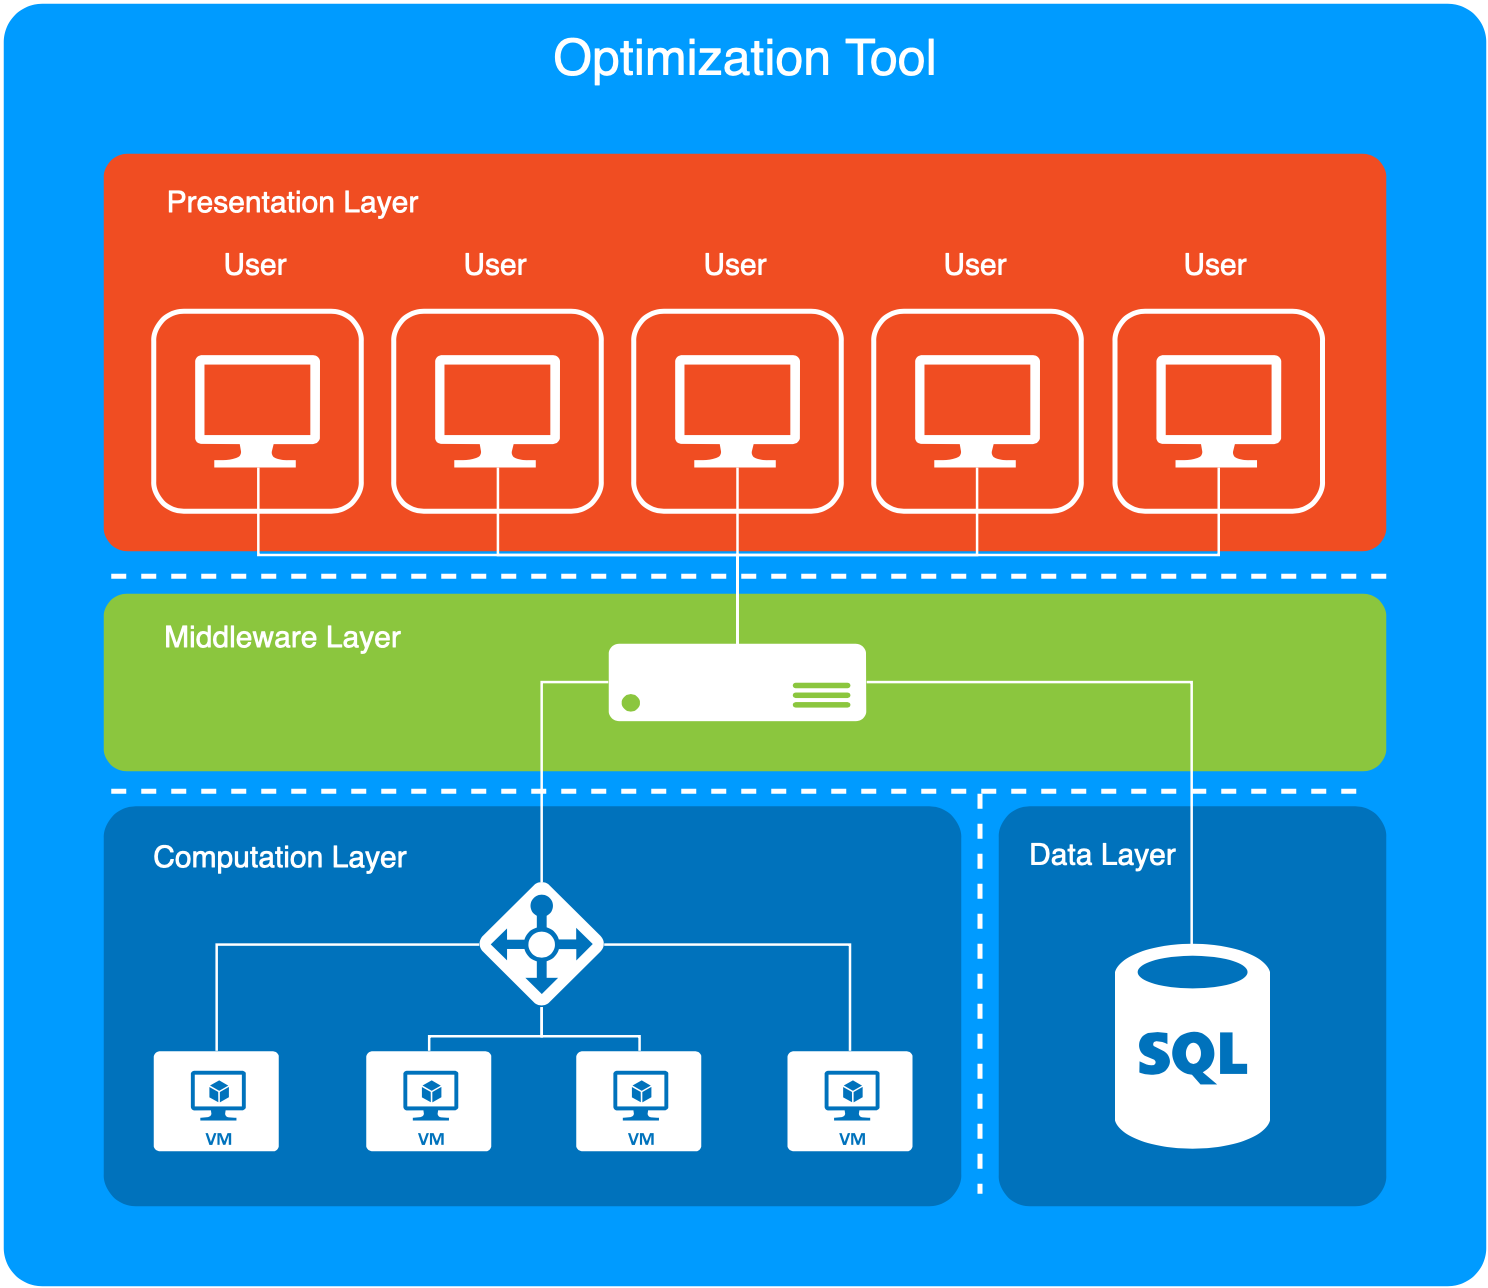
\includegraphics[width=0.5\textwidth]{pictures/ARCHITECTURE.png}
	\caption{The proposed architecture for scaling the optimization tool}
	\label{architecture}
	\flushleft\quad\quad\footnotesize{Source: Own Illustration.}
\end{figure}	

The computation layer is where the actual model is built and solved. It ideally consist of several worker units, possibly virtualized or containerized, which run the model code and a load balancing server queueing and assigning tasks received from the middleware layer via messages and relaying the returned solutions. It is currently implemented only rudimentary as shell script, that relays input and output data and launches the model code. The model code is written in the Julia programming language, which was chosen for its high performance \cite{JuliaMicroBenchmarks2018} and its focus on scientific computing. The model code also includes the data preprocessing code, which grants the user higher flexibility regarding the form and quality of her input data. It is integrated directly with the model itself, so the model can be used with different interfaces without the need to implement data preprocessing first (see 4.2). This does however impact performance, as preprocessing in the presentation layer would be distributed. \\
The data layer should ideally consist of an SQL database which allows the implementation of features in the presentation layer, that require a persistent state, such as user authentication or saved requests and solutions. It is accessed via the middleware layer. For all but the largest scale implementations there is no need to physically separate it from the middleware layer. The data layer and corresponding functionality are currently not implemented.
\\
The middleware layer coordinates communication between the users and the layers below. It is currently implemented as a simple node.js server \cite{fieldingArchitecturalStylesDesign2000} exposing a REST API \cite{fieldingArchitecturalStylesDesign2000} to the presentation layer.
\\
The presentation layer handles all user input and presents the results of the calculations conducted by the computation layer. It also handles all data processing required for presenting the data tu the user.  It is currently implemented as a Web Application using the React.js framework \cite{ReactJavaScriptLibrary2019} . 

\subsection{Workflow}
When the user enters data in the presentation layer, basic type checks are conducted. The input is then encoded as a JSON string \cite{crockfordIntroducingJSON}, which is sent as the payload of an HTML GET-Request \cite{fieldingArchitecturalStylesDesign2000} to the middleware layer. The middleware layer transfers the JSON string into the environment the model code is run in and launches the model code. The model preprocesses the received input. The preprocessing is configured with option parameters which are included in the input. Currently the model supports a number of preprocessing options:
\begin{itemize}
	\item Filling vector parameters, such as electricity prices or shiftable demand with a constant. 
	\item Adjusting the length of a number of vector parameters by cutting, if too long and looping, if too short.
	\item Adding noise to a number of vector parameters, by multiplying each value with a random number out of a normal distribution with a mean of 1.0. A variance can additionally be supplied.
	\item Normalizing the weights given to the discontinuous periods $s_i$.
\end{itemize} 
The model is then constructed and solved. For construction the Julia library "JuMP" \cite{JuMPJlModeling2019}is used, for solving the Gurobi commercial solver. \cite{GurobiOptimization} The model results are saved and transferred to the presentation layer via the middleware layer in a response to the GET-Request sent earlier. In the presentation layer the results are interactively visualized using the plotly visualization library. \cite{PlotlyJavascriptOpen2019} Currently a dispatch chart for each modeled household as well as two charts showing the generation and storage investment of each household are generated. In addition Key Performance Indicators (KPIs) such as the the levels of autarky and self-consumption or the average cost per KWh consumed are calculated to make different result easier to compare.

\newpage
\chead{\textit{Case Study}}	

\section{Case Study}
\subsection{Overview}
To demonstrate the viability of the designed model and of local microgrids, a limited case study is conducted. The location chosen is the small village of Morschenich in Northtrine-Westphalia, which is located in immidiate proximity to the lignite surface mine of Hambach. According to current plans of RWE, the owner and operator of the mine and the state of Northrine-Westfalia, the village is due to be razed and the population resettled by the year 2024, when the mining activities are expected to reach the village. \cite{rwepowerRahmendatenMorschenichGemeinde2018}\cite{gemeindemerzenichUmsiedlungMorschenich}
\begin{figure}[H]
	\centering
	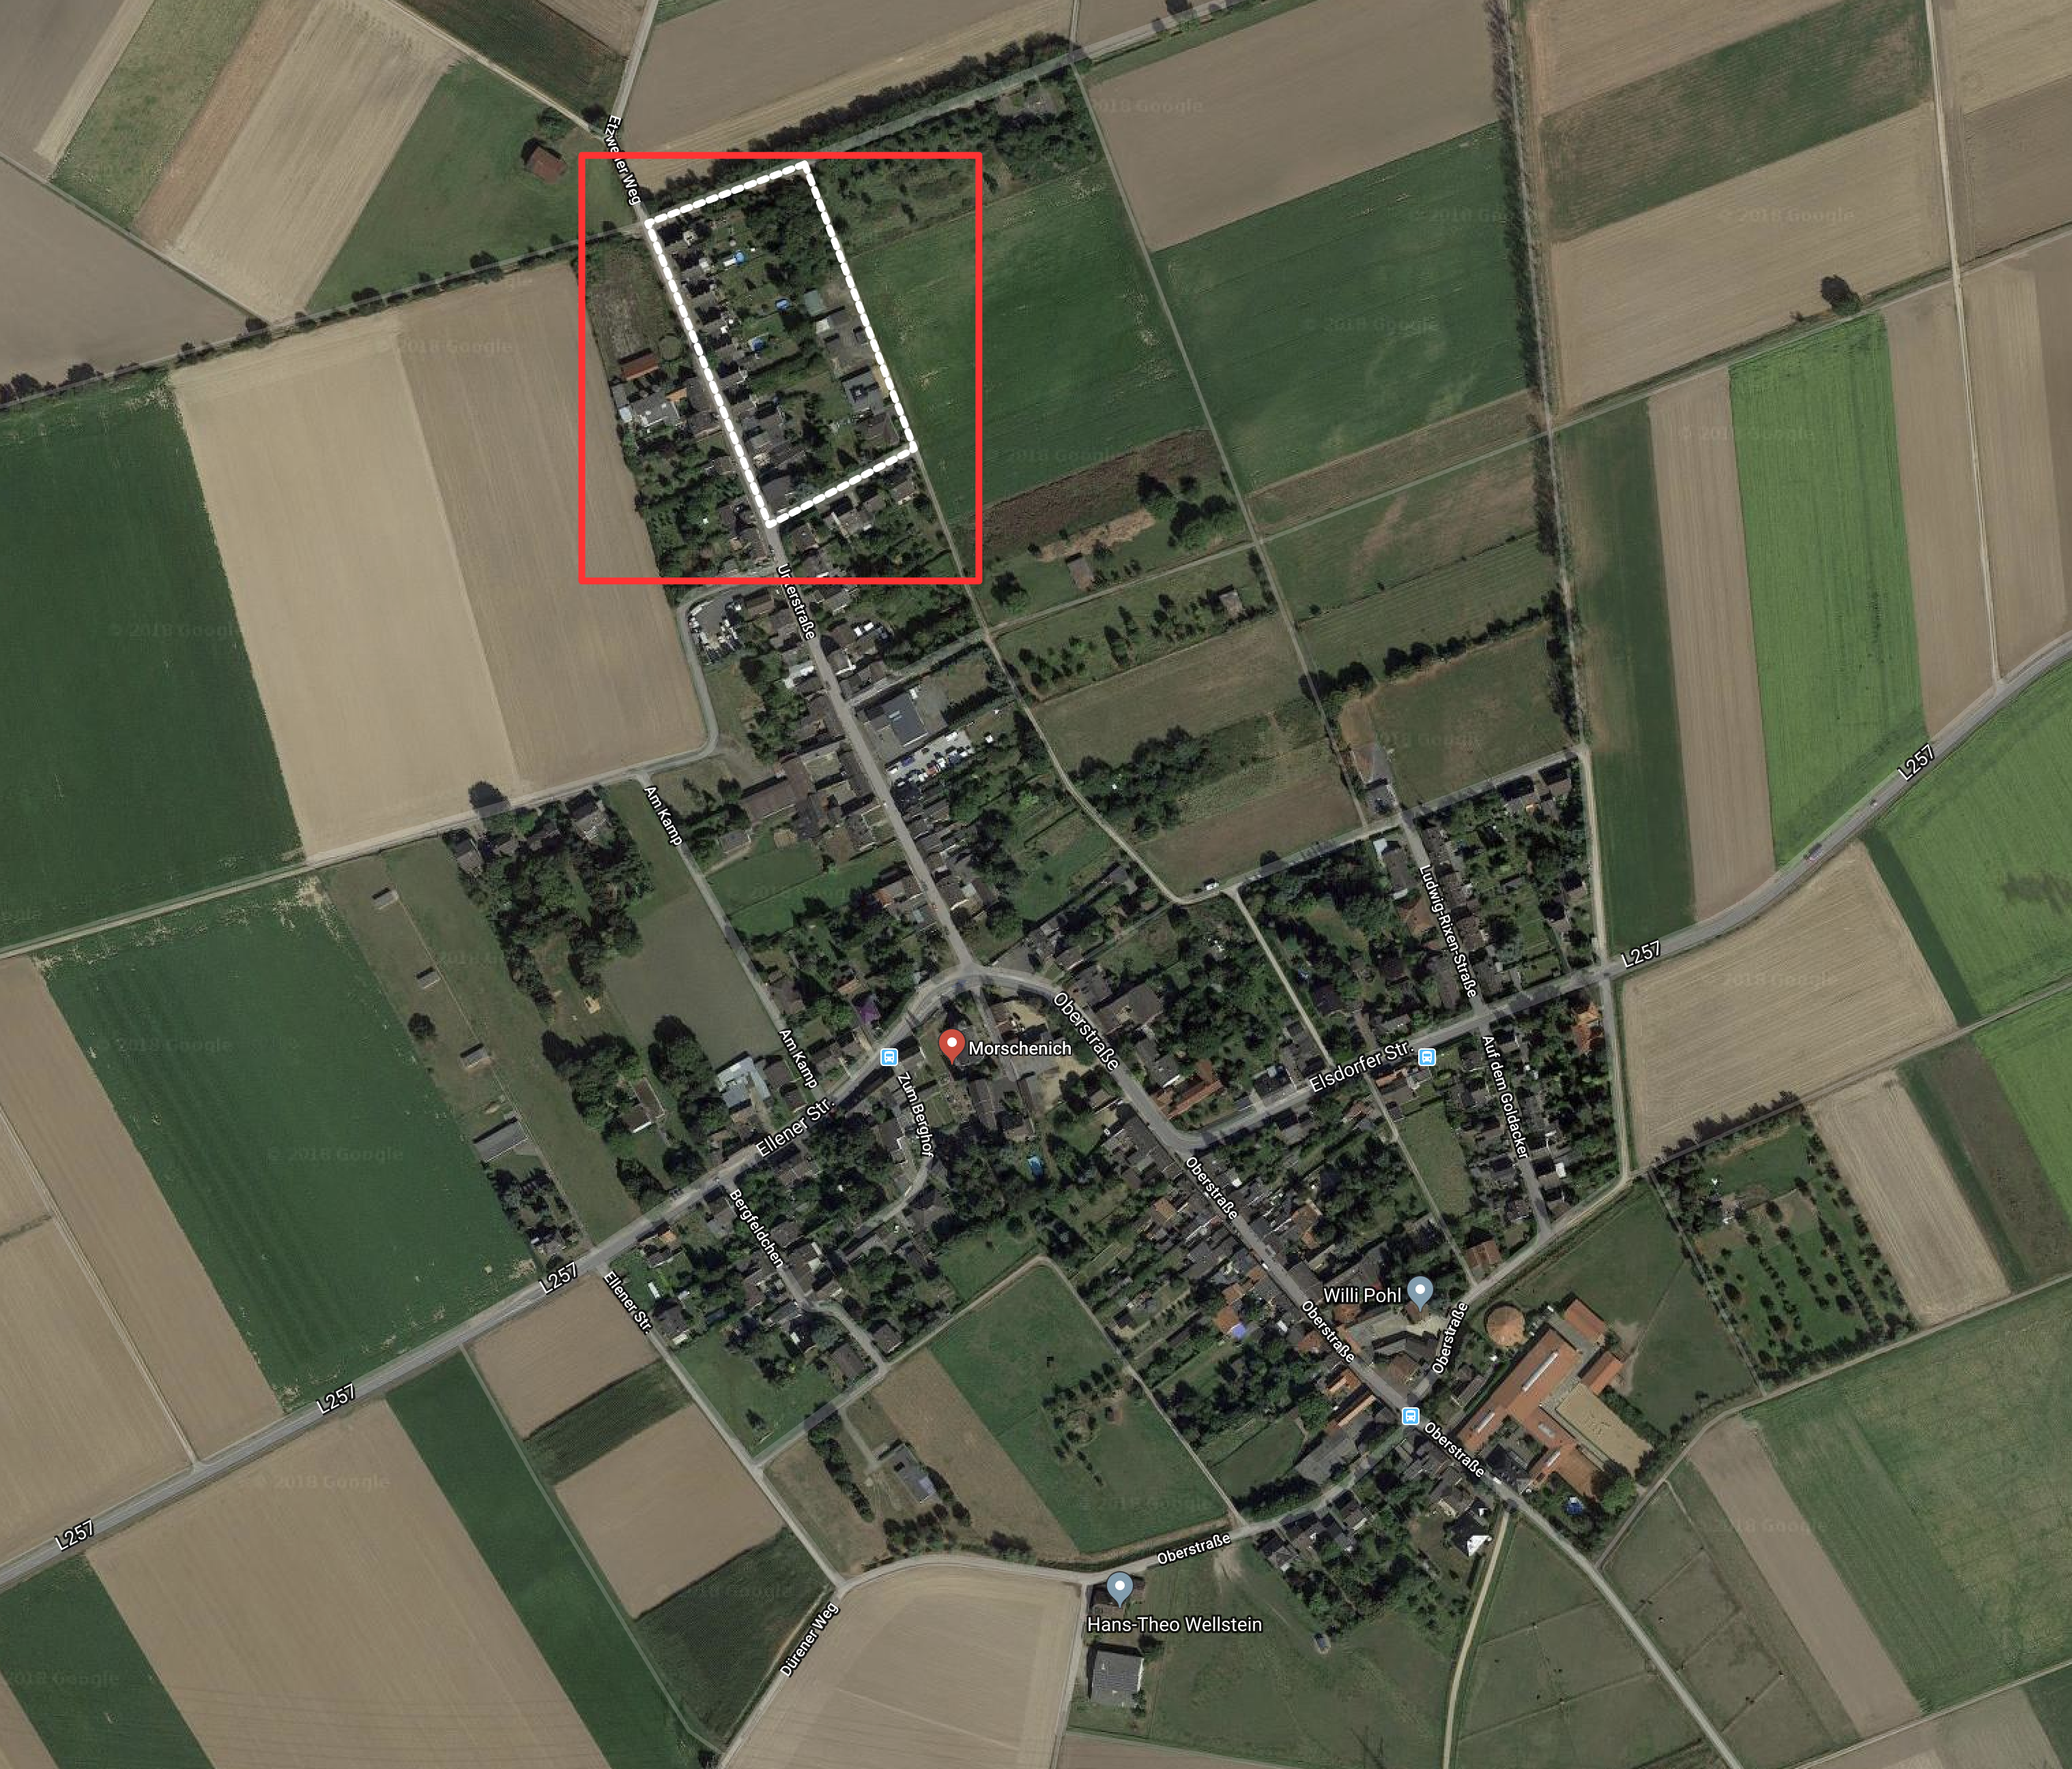
\includegraphics[width=0.75\textwidth]{pictures/Morschenich.png}
	\caption{The village of Morschenich}
	\label{morschenich}
	\flushleft\quad\quad\footnotesize{Source: Google Maps.}
\end{figure}	
Although the resettlement process has already begun and the village 'Morschenich-Neu' is under construction several kilometers away, there are as of the date of writing still several hundred inhabitants remaining in Morschenich, including some Syrian war refugees, who have been accommodated in abandonden houses of families already been resettled.\cite{bauerAbgrundtief2018}
\\
The case study will focus on the northern part of Morschenich, where several housing- and two commercial units are located in block as indicated by the white line in Figures 2 and 3. 

\begin{figure}[H]
	\centering
	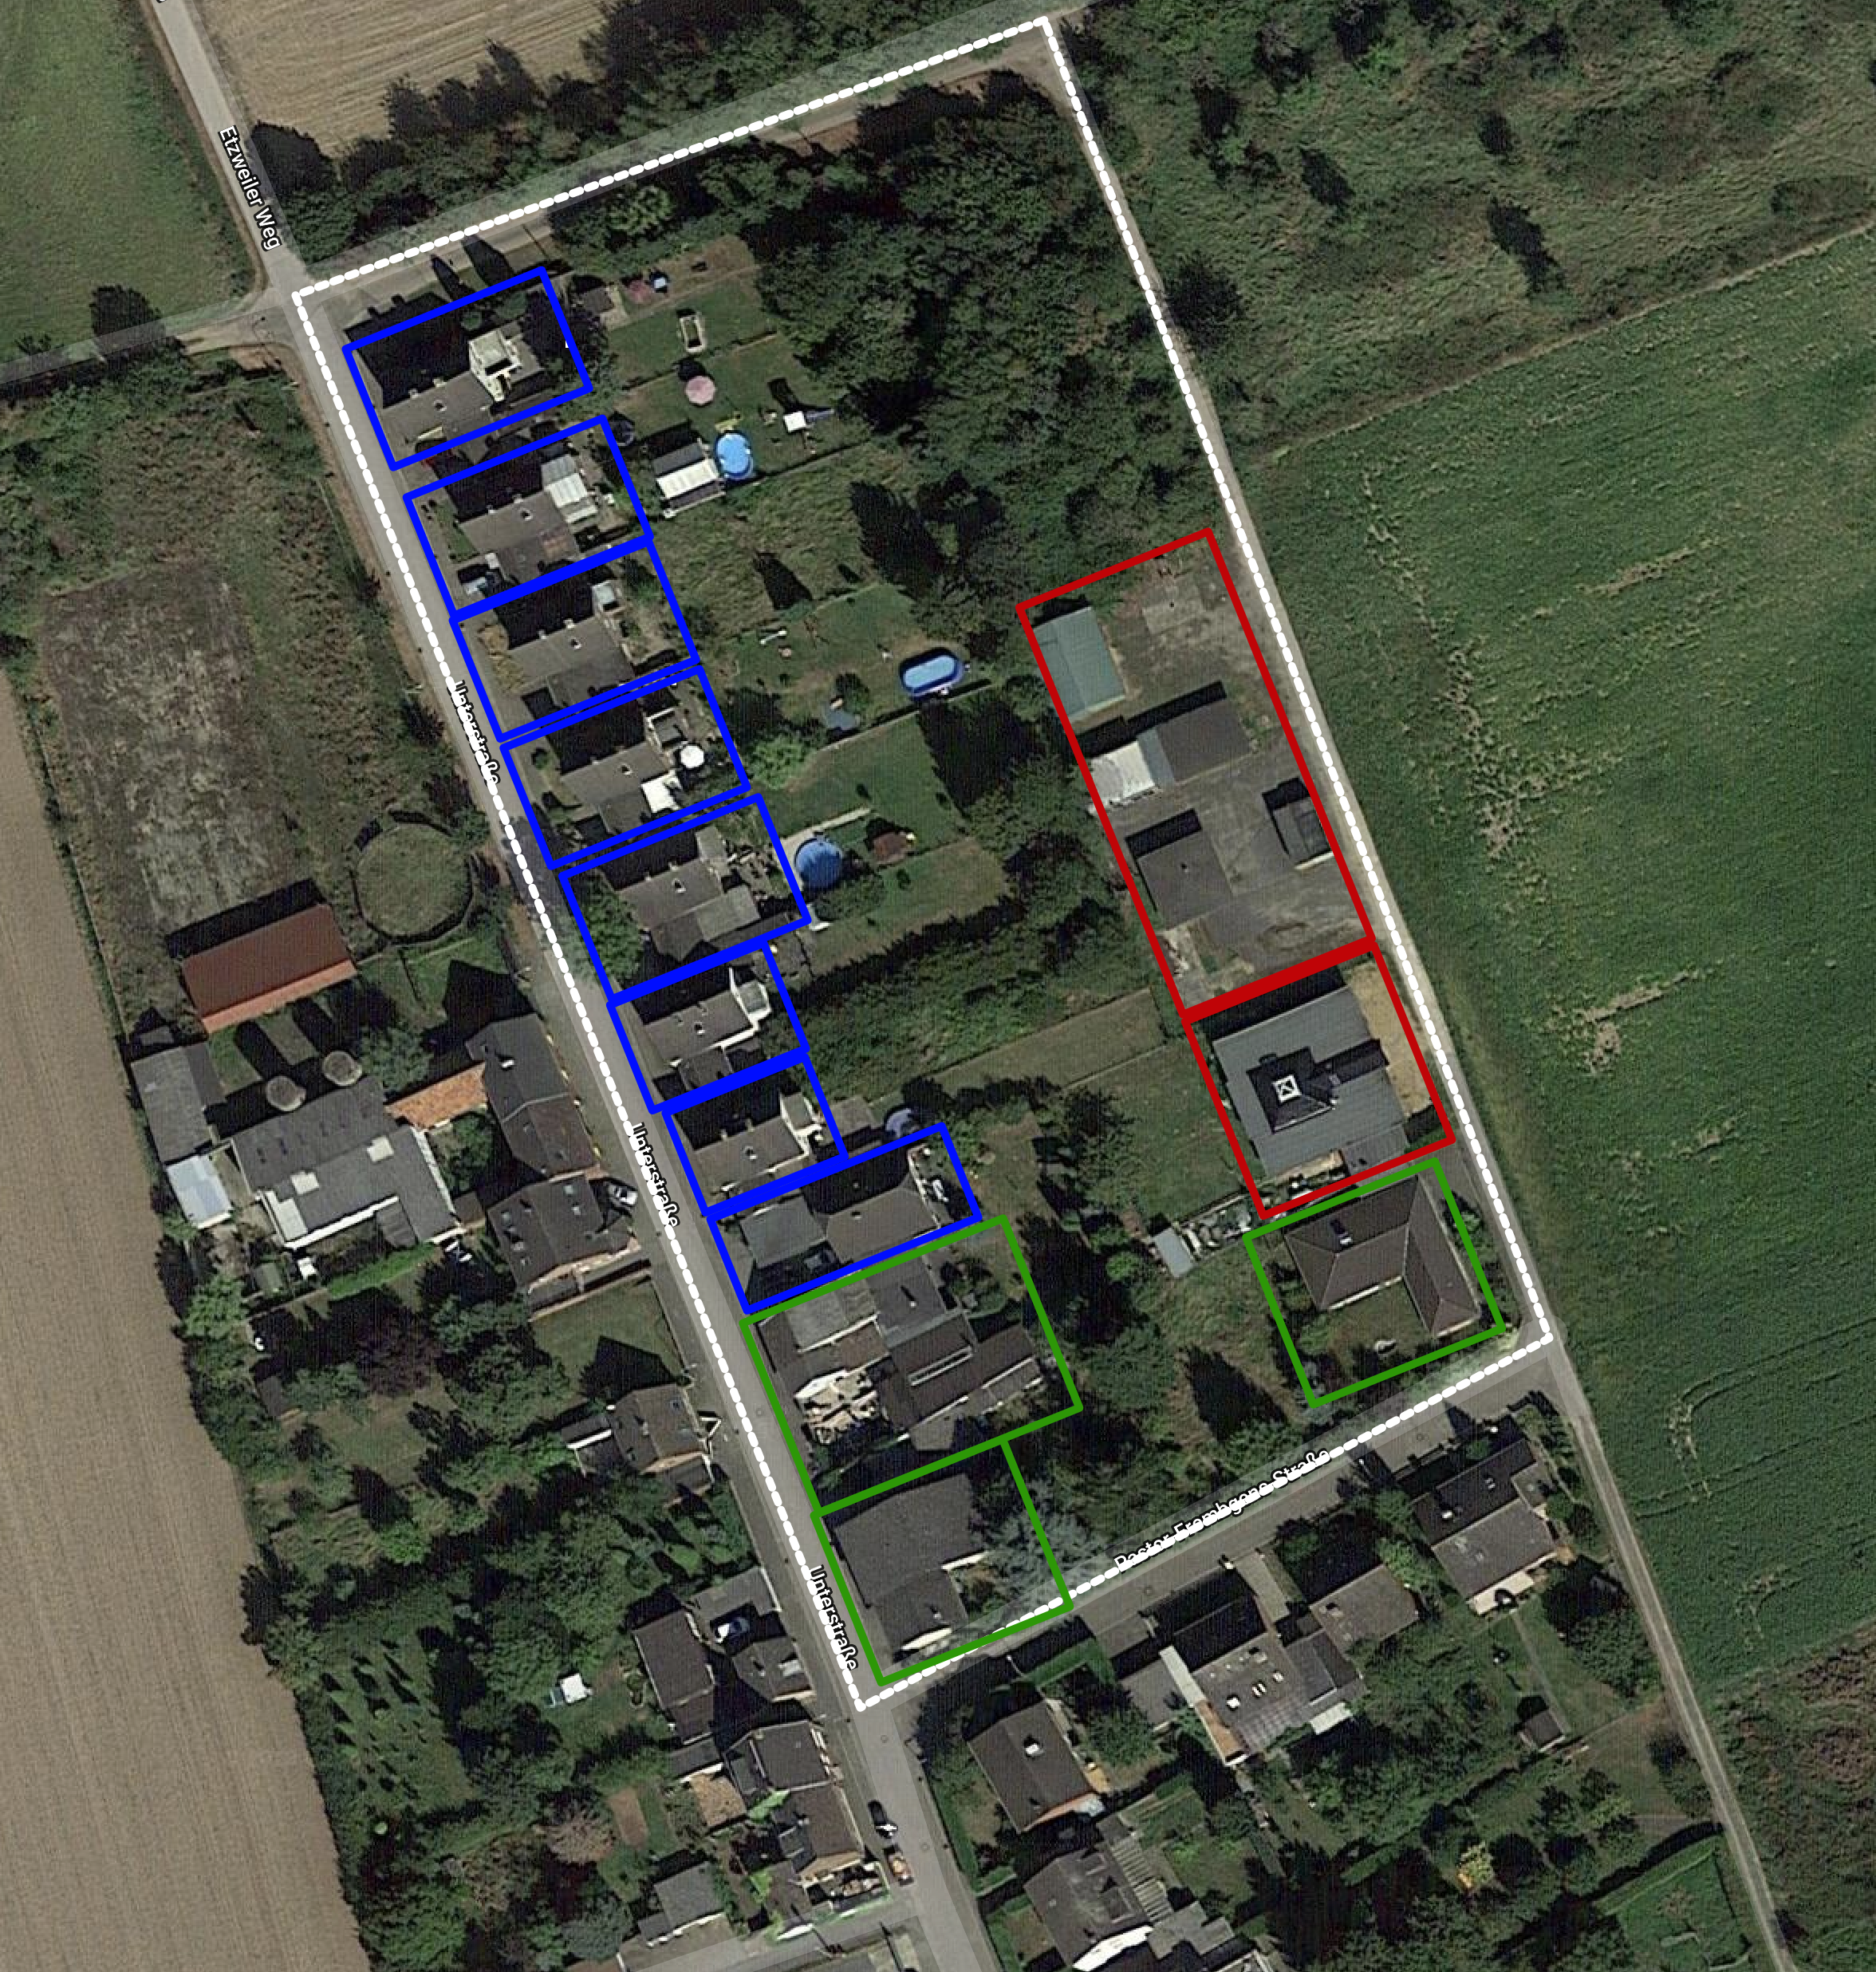
\includegraphics[width=0.75\textwidth]{pictures/Detail_Layout.png}
	\caption{A detailed view of the chosen location.}
	\label{morschenich_detail}
	\flushleft\quad\quad\footnotesize{Source: Google Maps.}
\end{figure}	

In figure 3 all buildings in the area designated for the case studies proposed microgrid have been marked with coloured boxes. Blue boxes represent small residential units, while green boxes indicate larger residential and red boxes commercial units.
\\
The case study will examine the business case of the establishment of an autonomous microgrid in the selected area. Therefore we model investment decisions and dispatch for three discontinuous periods of one week each to reflect the different conditions encountered throughout the year. The buildings designated will be assumed to be the participants of the considered microgrid. The different classes of buildings are modelled with different parameters to accurately represent their distinct sizes and uses.

 The following sections will document the assumed input parameters the model requires for the calculation of a base scenario and how they were derived. To properly function the model requires meteorological data for constraints on intermittent power generation, as well as data on investment options, household demand and grid supply. The final section will introduce a number of further scenarios in which some of the assumptions are changed.






\subsection{Meteorological Data}
An hourly profile of solar the capacity factor for a pv installation in Morschenich is sourced from \cite{pfenningerLongtermPatternsEuropean2016}. From the profile, which includes an entire year of data, three samples are extracted: One 144 hour sample representing the transitional season, e.g. spring and fall and two 72 hour samples representing summer and winter. The difference in length is not relevant for use in the model, as the data preprocessing only uses these profiles as input for generating the profiles used in the optimization itself (see section 4). The resulting vector of values is used as the parameter $GEN_1 \hookrightarrow maxFl$, which is interpreted as the maximum input flow for the solar pv installation. In addition the parameter $EFF_{el}$ is set to 1.0, which makes the model effectively treat the vector as a capacity factor.

\subsection{Investment Options}
To test the different implementations of discrete and linear investment options the case study incorporates two linear-scaling generation devices as possible investments, as well as two discretely-scaling storage devices. The generation devices consist of a photovoltaic system as a renewable option and a combined heat and power fuel cell, as a conventional, though decentralised and highly efficient option. It is further capable of using biofuels, which can be expressed through higher fuel prices. 
\begin{table}[H]
	\centering
	\caption{Parameters describing the generation technologies}
	\begin{tabular}{lllll}
		\hline
		\textbf{Parameter}			& \textbf{Name}			& \textbf{Unit}			& \textbf{Value}	&\textbf{Reference}     \\ \hline
		\textit{Photovoltaic System} & $GEN_1$ & & &\\
		Installation Cost           & $C_{Cap}$     		& \euro $KW^{-1}$  		& 1200				& Estimate based on \cite{wirthAktuelleFaktenZur2018}, \cite{SolarmoduleEBay2018}, \cite{ModulePriceIndex2018}   \\
		Maintenance Cost            & $C_{OpFix}$     		& \euro $KW^{-1}yr^{-1}$& 50				& Estimate \\
		Fuel	 Cost           			& $C_{OpVar}$     		& \euro $KWh^{-1}$   	& 0.0			& no sun taxes ... yet  \\
		Lifetime                    & $T_{Life}$     		& $yr$  				& 25 				& \cite{wirthAktuelleFaktenZur2018}   \\
		Electric Efficiency         & $EFF_{el}$     		& $\%$  				& 100				& included in $maxFl$      \\
		Performance Ratio           & $PR$     		& $\%$  				& 85				& \cite{wirthAktuelleFaktenZur2018}   \\
		Maximum Input Flow  			& $maxFl$     		& $KW$ 		 			& see section 5.2				& based on insolation   \\
		\hline
		\textit{CHP Micro Fuel Cell} & $GEN_2$ & & &\\
		Installation Cost           & $C_{Cap}$     		& \euro $KW^{-1}$  		& 3500 				& Estimate based on \cite{LAUINGER201624}    \\
		Maintenance Cost            & $C_{OpFix}$     		& \euro $KW^{-1}yr^{-1}$& 175				& Estimate based on \cite{LAUINGER201624}   \\
		Fuel	 Cost           			& $C_{OpVar}$     		& \euro $KWh^{-1}$   	& 0.0608			& \cite{NaturalGasPrices2018}   \\
		Lifetime                    & $T_{Life}$     		& $yr$  				& 15 				& \cite{LAUINGER201624}    \\
		Electric Efficiency         & $EFF_{el}$       		& $\%$  				& 60				& \cite{BlueGENWorldsMost2018}   \\
		Performance Ratio           & $PR$     		& $\%$  				& 100				& no additional penalties  \\
		Maximum Input Flow  			& $maxFl$     		& $KW$ 		 			& 999				& no restrictions  \\
		\hline
	\end{tabular}
\end{table}

The storage investment options given are two differently sized Lithium Ion batteries: A 4 KWh option manufactured by Victron Energy and a 13.5 KWh option manufactured by Tesla. While the two generation devices are hypothetical, these storage devices can actually be bought, which leads to lower error due to false assumptions and linearisation of non-linear relationships (such as storage size and price). This the main advantage discrete modelling of investment options has over linear modelling.

\begin{table}[H]
	\centering
	\caption{Parameters describing the storage technologies}
	\begin{tabular}{lllll}
		\hline
		\textbf{Parameter}			& \textbf{Name}			& \textbf{Unit}			& \textbf{Value}	&\textbf{Reference}     \\ \hline
		\textit{Li-Ion Battery 1} & $dST_1$ & & &\textit{Tesla Powerwall} \\
		Usable Capacity				   & $CAP$ 		& $KWh$ 				& 13.5 				& \cite{PowerwallTesla2018} 	\\
		Installation Cost              & $C_{Cap}$        	& \euro 				& 10000				& Estimate based on \cite{PowerwallTesla2018}   \\
		Lifetime			               & $T_{Life}$       	& $yr$  				& 10 				& Estimate based on \cite{PowerwallTesla2018} \\
		Roundtrip Efficiency           & $EFF_{+-}$     	& $\%$  				& 90				& \cite{PowerwallTesla2018}   \\
		Max. charging power            & $maxP_+$    	& $kW$  				& 4.6 				& \cite{PowerwallTesla2018}      \\
		Max. discharging power         & $maxP_-$     	& $kW$   				& 4.6 				& \cite{PowerwallTesla2018}      \\
		Initial State of Charge        & $-$     	& $\%$  				& 100 				& Assumption   \\
		Terminal State of Charge       & $-$     	& $\%$  				& 100 				& Assumption   \\
		\hline
		\textit{Li-Ion Battery 2} & $dST_2$ & & & \textit{Victron Energy Lithium HE Batterie} \\
		Usable Capacity				   & $CAP$ 		& $KWh$ 				& 4 				& based on \cite{LithiumIonenHEHigh2018} considering depth of discharge\\
		Installation Cost              & $C_{Cap}$     	& \euro  				& 5000				& Estimate based on \cite{VictronEnergyLithium2018}   \\
		Lifetime			               & $T_{Life}$     	& $yr$  				& 10 				& Estimate based on \cite{LithiumIonenHEHigh2018}   \\
		Roundtrip Efficiency           & $EFF_{+-}$      	& $\%$  				& 92 				& \cite{LAUINGER201624}    \\
		Max. charging power            & $maxP_+$    	& $KW$  				& 4.8				& \cite{LithiumIonenHEHigh2018}    \\
		Max. discharging power         & $maxP_-$     	& $KW$   				& 7.2				& \cite{LithiumIonenHEHigh2018}    \\
		Initial State of Charge        & $-$     	& $\%$  				& 100 				& Assumption	   \\
		Terminal State of Charge       & $-$    	& $\%$  				& 100 				& Assumption   \\	
		\hline
	\end{tabular}
\end{table}

\subsection{Demand}
As the case study distinguishes between three types of buildings, three demand profiles where compiled. Each profile is made up of three hourly load vectors spanning one or several days. Demand vectors for the two types of residential units are sourced from \cite{ReferenzlastprofileUndMehrfamilien2008}. The choice was made because these profiles are specifically created for optimization of decentralized generation. They are samples of measurements taken on several houses and therefore feature a much higher variability than standard profiles, which usually are averages of many measurements. In the context of this case study it is critical to accurately reflect this high variability, which a microgrid can do a lot to manage. For the commercial units profiles where sourced from the association of the German power industry (BDEW) \cite{fuenfgeldAnwendungRepraesentativenVDEWLastprofile2000}\cite{StandardlastprofileStrom2017}. These are standard profiles specifically from commercial consumers. The samples were of varying sizes of one to several days, to reflect the approximate ratios of occurences of the different model days provided for our particular meteorological region. They were further preprocessed by the model itself. The noise filter of the model was provided with a variance value of 0.25 for the smaller residential households and a variance of 0.15 for the larger residential and commercial buildings (see 4). This additional noise is crucial in distinguishing the demands of different instances of one household type from one another, as would occur in reality. Furthermore it makes the load profile more realistic, when scaled beyond its original length, since it makes the repeated profile differ notably.(see 4)
\\
For the residential buildings it is assumed that at any time 10 percent of loads can be curtailed at a flat renumeration rate of 0.35\euro per KwH. A further 20 percent of total loads are assumed to be shiftable at a flat rate of 0.15\euro per KwH per hour shifted. The remaining 70 percent of loads are deemed essential. The commercial units can also shift up to 20 percent of their load for 0.15\euro per KwH per hour, but no curtailment is allowed.

The profiles are scaled for the total yearly demand of the smaller residential buildings to be around 5000 KWh. The multi-family residential and commercial buildings' profiles are scaled to a yearly demand of approximately 10000 KWh and 16000 KWh respectively. 

\subsection{Grid Supply}
For the base scenario the grid supply is assumed to be capped at a constant value of 500KW, which guarantees that all supply can be met solely by the grid. It is further assumed that the price of this energy is set at 0.3\euro at any time\cite{Monitoringbericht20182018}. The feed in tariff is assumed to be constant at 0.08\euro and the feed-in is capped at a constant 20KW.

\subsection{Further Assumptions}
To keep the model from trading randomly inside the microgrid, a trade fee of 0.001\euro per KWh is imposed on all trade within the microgrid.\\
To accurately reflect the prevalence of the weather conditions and demand profiles represented by the three seasonal periods modelled the summer, winter and transitional period have been weighed with the factors 169, 81 and 115, respectively. These factors are normalized during preprocessing (see 4) and all cost incurred during each period is multiplied with the normalized corresponding weight. The weights have been chosen according to the prevalence of different weather conditions in the meteorological region of Morschenich \cite{ReferenzlastprofileUndMehrfamilien2008}.

\subsection{Results}
Surprisingly, even in the base scenario, the microgrid seems to be commercially viable, as an autarky level of 94 percent is reached. Investment is heavily biased towards Fuel Cells (see figure 4), which are installed at a smaller capacity than pv installations but operate at a capacity factor of up to 100 percent versus around 12 for pv. Therefore, most power is generated by flexible gas fuel cells (dark blue) only supplemented by a small amount of pv generation (light blue).\\
The ratio of fuel cell versus pv installation varies depending on the total amount and temporal distribution of demand: While the small residential residences install mostly fuel cells, the larger residential units invest in an almost equal capacity of both, while the commercial units install a lot more pv capacity than fuel cells. This is probably to keep the self-consumption ratio high, while minimizing trade, which is cheap but not free. The commercial units have by far the highest demand during midday which can be served by solar energy without demand shifting or storage.
\begin{figure}[H]
	\centering
	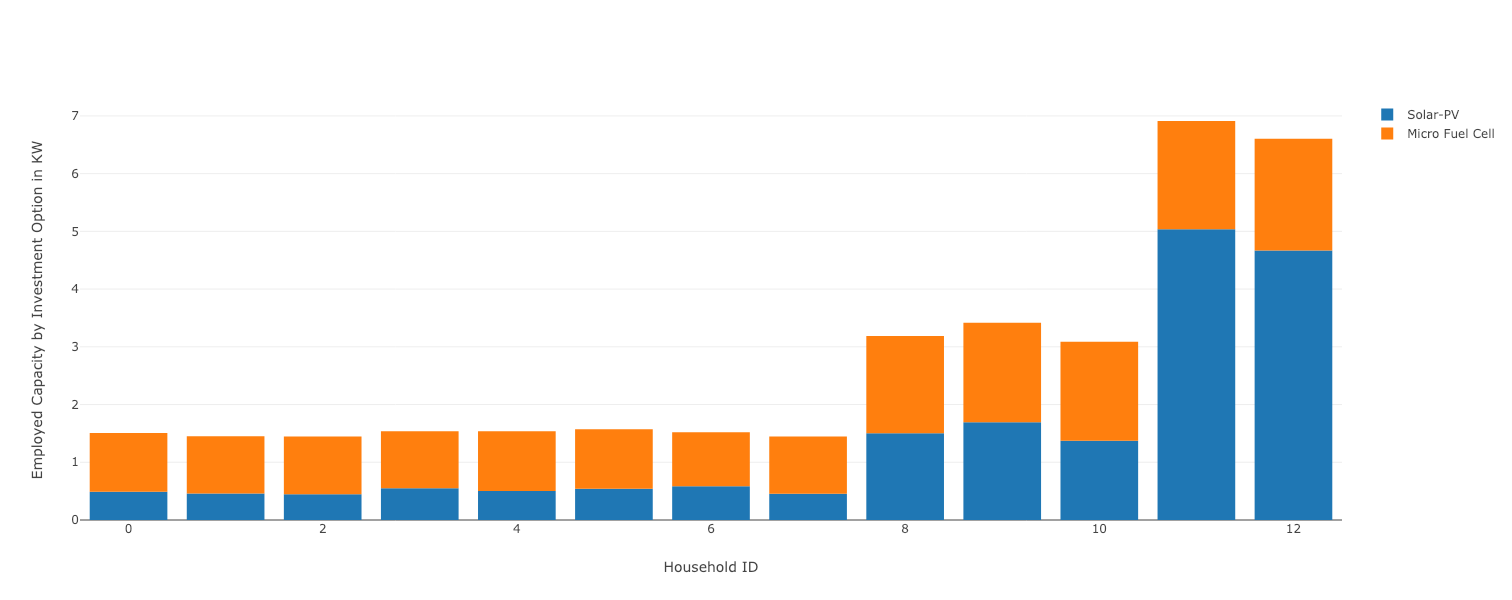
\includegraphics[width=1\textwidth]{pictures/INV_GEN_Base.png}
	\caption{Generation investment in the base setup of the case study}
	\label{gen_investment_base}
	\flushleft\quad\quad\footnotesize{Source: Own Model User Interface}
\end{figure}
With this setup the model stays at a self-consumption rate of 100 percent, as feed-in renumeration seems to be smaller than the marginal cost of generating power with the fuel cells. Furthermore no storage is needed to achieve these levels of autarky and self-sufficiency. \\
As can be observed in figures 5 and 6 trading (orange and pink) is heavily utilised for balancing, as the load profiles of participants differ enough to enable this. Also load shifting (green and purple) is sporadically used (see figures 5 and 6), but rarely loads are shifted for more than one hour.

\begin{figure}[H]
	\centering
	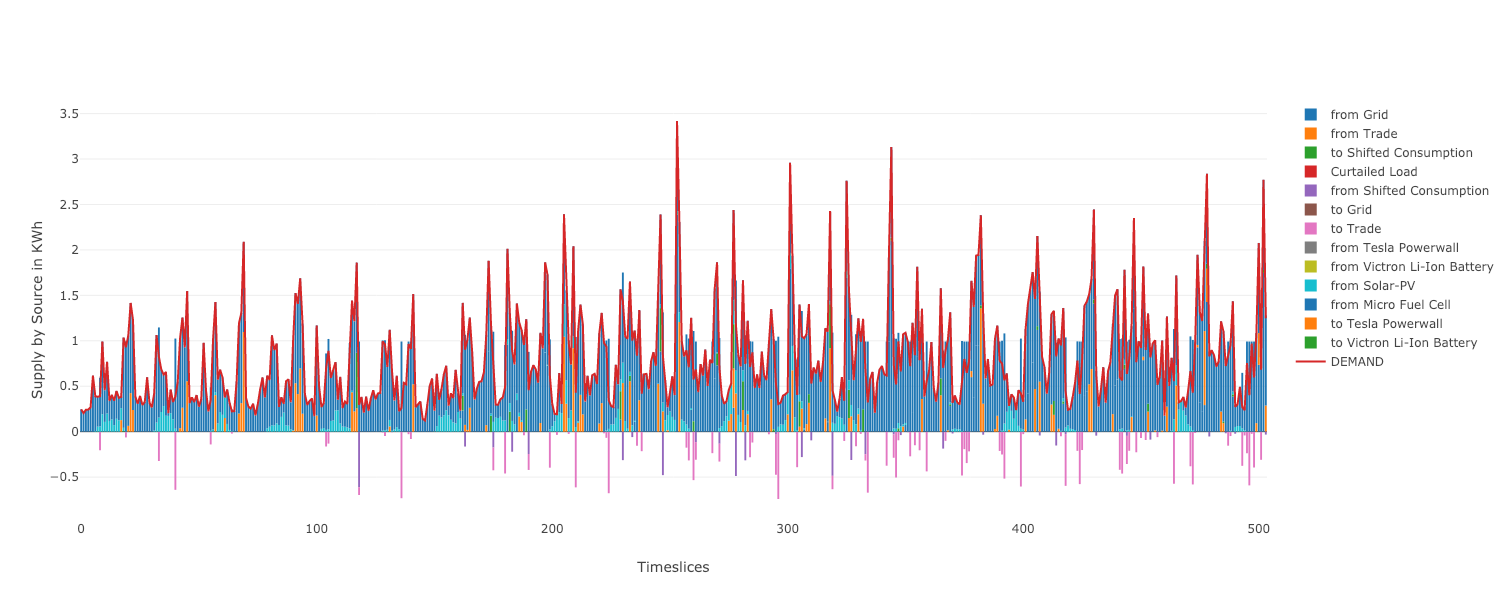
\includegraphics[width=1\textwidth]{pictures/RES_1_Base.png}
	\caption{The dispatch of a residential building in the base setup of the case study}
	\label{residential_dispatch_base}
	\flushleft\quad\quad\footnotesize{Source: Own Model User Interface}
\end{figure}	

The only use of the use of grid energy (also dark blue, but below orange and light blue) occurs during the winter week (the last third of the dispatch chart), when generation and internal dispatch are insufficient to meet peak demand, most likely due to a lack of irradiation (see Figure 7). This indicates that the levelized cost of solar energy is significantly below that of the electricity generated by fuel cells, as it would otherwise be cheaper to satisfy demand entirely with them instead of adding solar and as a consequence having to rely on some grid imports during winter.

\begin{figure}[H]
	\centering
	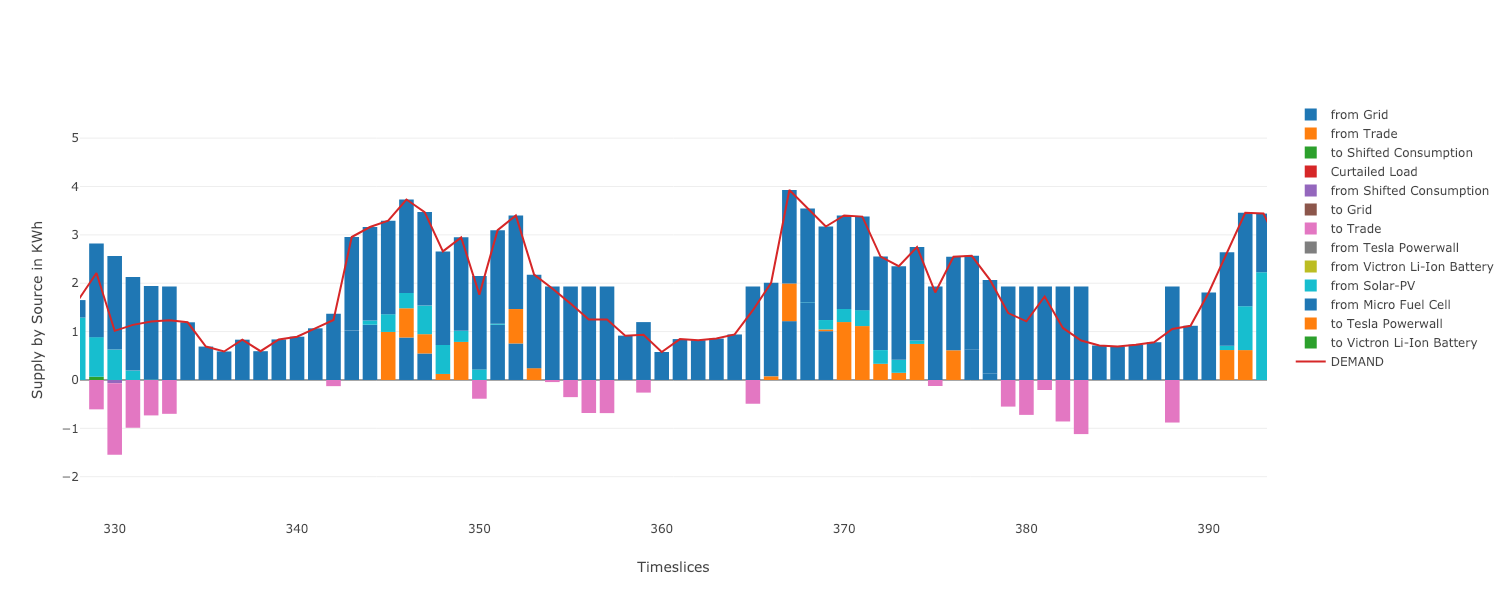
\includegraphics[width=1\textwidth]{pictures/COM_2_ZOOM_Base.png}
	\caption{The dispatch of a commercial building in detail for two winter days}
	\label{commercial_dispatch_base}
	\flushleft\quad\quad\footnotesize{Source: Own Model User Interface}
\end{figure}	

Overall the result is surprisingly cheap, with the average cost per KWh being at about 0.164 \euro and the total cost at approximately 1259.624 \euro.\\
The model solves in approx. 4-6 minutes on a macOS 10.14 system with the Gurobi Commercial Solver and a 3.3Ghz Quad-Core Intel Core i5 processor with 24GB of 1867MHz DDR3 RAM.

\subsection{Sensitivity Analysis}
To test the validity and robustness of the solution obtained above, a sensitivity analysis is conducted. 

To test the importance of the use of fuel cells for the result and its robustness, first the price of gas is raised by 50 percent. This could reflect the $CO^2$ neutral use of more expensive biogas or the insecurity of the price of fossile fuels in general, as the investment horizon considered in the case study is up to 25 years.
\begin{figure}[H]
	\centering
	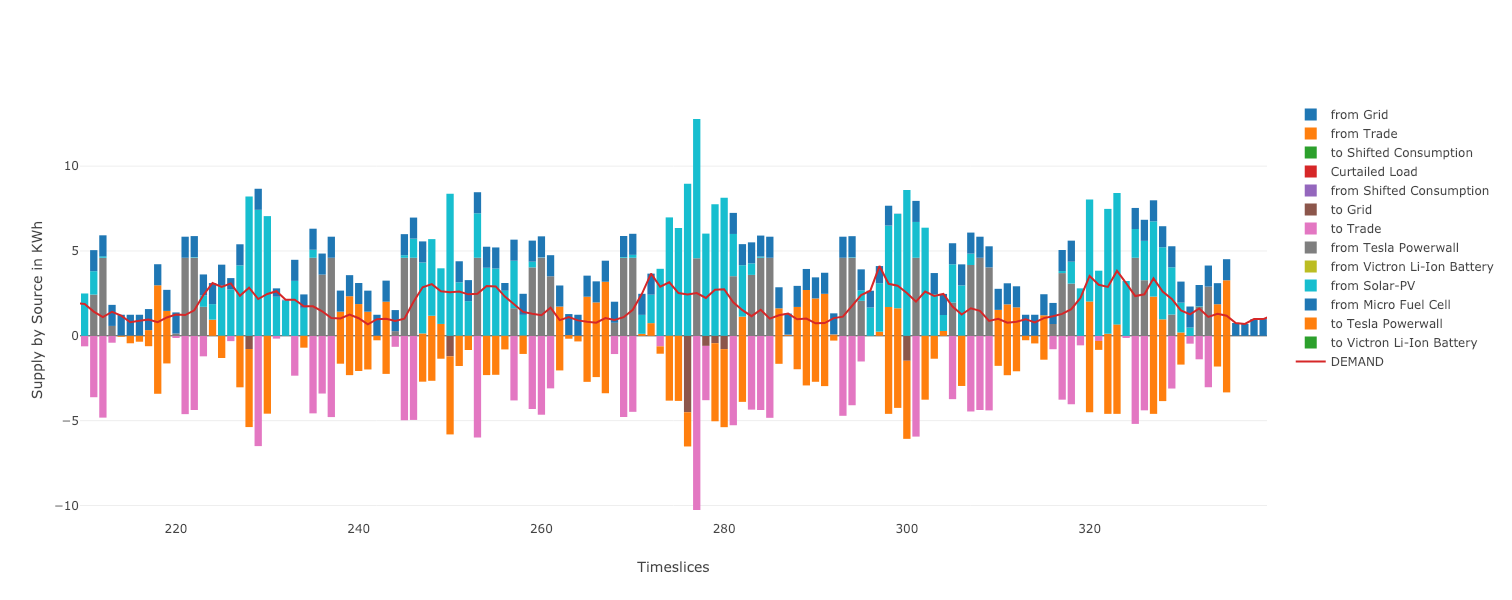
\includegraphics[width=1\textwidth]{pictures/SCEN_1.png}
	\caption{Effects of a gas price increase of 50 percent}
	\label{commercial_dispatch_base}
	\flushleft\quad\quad\footnotesize{Source: Own Model User Interface}
\end{figure}	

The increased gas price results in a drop of installed fuel cell capacity by around a quarter. Pv deployment consequently increases by over 300 percent. One of thee commercial buildings, in addition to 17.7 KWp of pv is equipped with a Tesla Powerwall, which is utilized heavily to store solar energy which is traded to the microgrid during the evening (see figure 7). Autarky remains high at 92 percent, while self consumption drops slightly to 96 percent. The grid is still not utilized a lot since the average price per KWh at 0.199 \euro is still well below grid power prices. Still the objective value rises approx. 20 percent to 1524.547 \euro.

Another factor which seems critical to the base result is the reliance on trading. To test the robustness of trading, the price per traded KWh of electricity is raised from a merely symbolic 0.001\euro to 0.03\euro. This could be considered the cost of maintaining the infrastructure of the grid, or the energy lost in cross-microgrid transactions.
\\
This has only a negligible effect, as the objective value is only raised by about 10 \euro. Raising the fee to 0.06 \euro. per KWh has a similarly small effect, raising the objective value by another 18 \euro. Another incrase to 0.09 \euro fails to have a much greater impact at an objective value of approx. 1293 \euro. 

Another possibility is a change in the price of pv panels and batteries in the coming years. To test the effect these changes could have on the optimal result, the base case is altered by reducing the investment price of pv installations by 25 percent and the investment price of storage by 35 percent. This has a simnilar effect to increased gas prices, in that fuel cell deployment falls, whereas pv installations increase. Additionally, as before, one Tesla Powerwall is installed by a commercial entity. The effect on the objective value however is not significant, as it is only decreased by 46\euro or 0.005\euro per KWh. Adding the 50 percent increased gas prices to alterations results in a total of 64 KWp pv installation, but only a single Powerwall, which seems to suffice, as self-consumption is still at 92 percent. The average electricity price rises to 0.19 \euro. Decreasing battery prices by 50 percent relative to the base case results in the. installation of a second Powerwall in one of the multi-family residential buildings. The solution however, is hardly superior at 0.188 \euro per KWh. 
\\\\
Finally, a major weakness of the base cases result is the linear scaling of the price of generation technology, which leads to installation of small capacities throughout the microgrid. In reality this would be very expensive, since the prices do not in fact scale linearly. To test the robustness to non-linear generation options, we convert both generation options to discrete investments. The pv installation will only be available in increments of 5 KWp and the Fuel Cell in increments of 2.5 KWp.\\\\ 
	The test is run with a 15 min time limit, as it does not terminate in a reasonable amount of time otherwise. The gap to optimality after this period is at 0.26 percent or approx. 4 \euro. 

\begin{figure}[H]
	\centering
	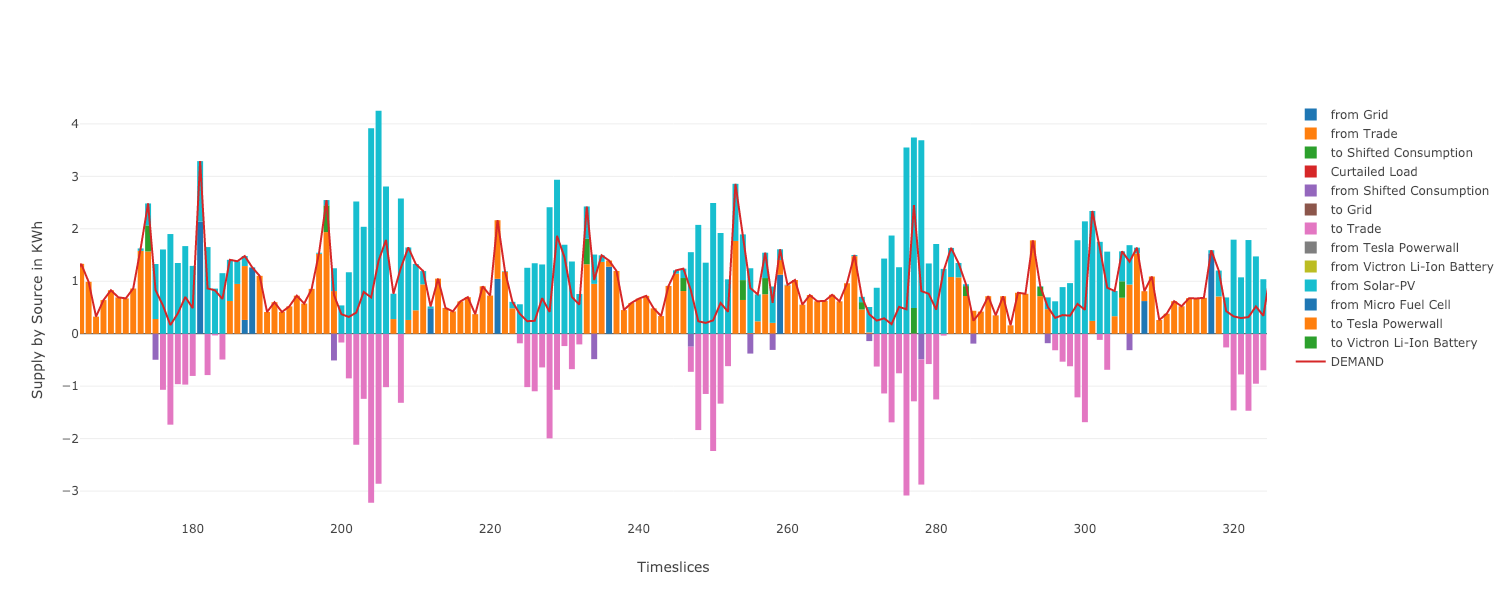
\includegraphics[width=1\textwidth]{pictures/RES_2_DISC.png}
	\caption{A household with a pv installation under an all-discrete constraint}
	\label{commercial_dispatch_base}
	\flushleft\quad\quad\footnotesize{Source: Own Model User Interface}
\end{figure}	

	While the objective value at approx. 1257 \euro does not differ from the base case by a lot, the added constraints lead to a very different behaviour. Households are now clearly seperated into producers and consumers, some generating power with a pv installation, some with a fuel cell (see fig. 9 and 10). This leads to a strong increase in trading activity between the households as the microgrid tries to distribute the now more centralized generation.
	
\begin{figure}[H]
	\centering
	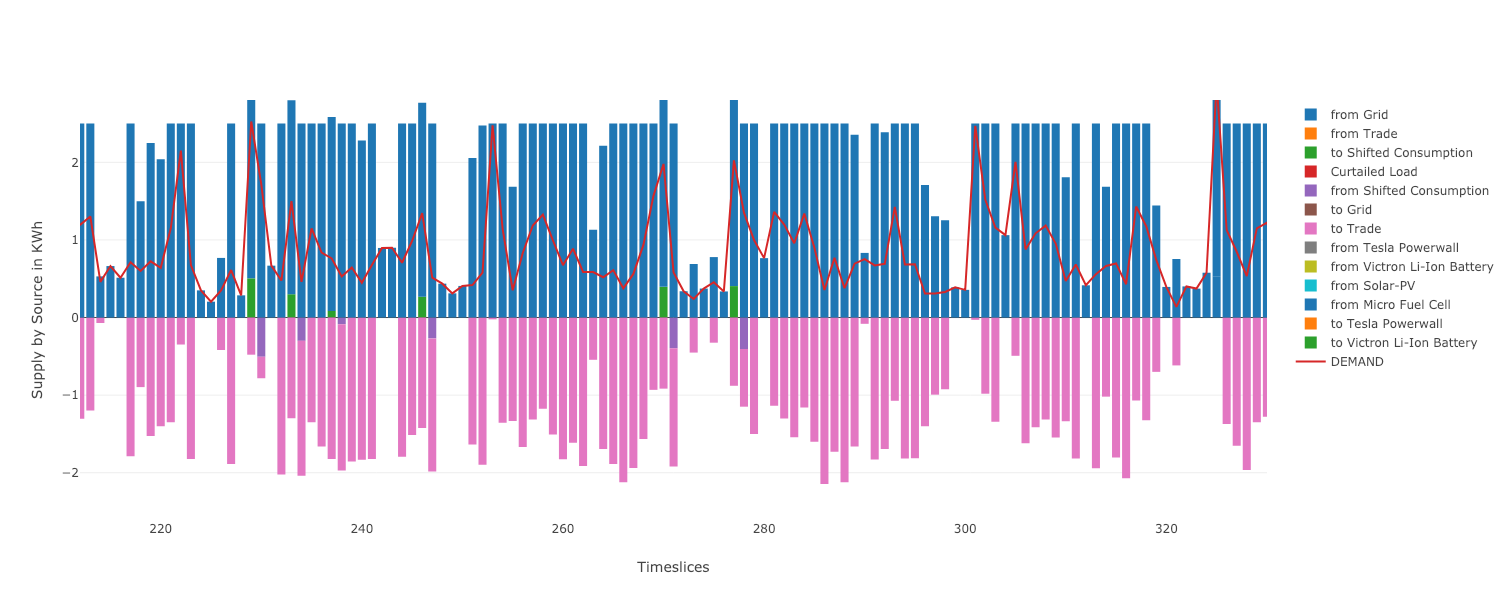
\includegraphics[width=1\textwidth]{pictures/RES_8_DISC.png}
	\caption{A household with a fuel cell under an all-discrete constraint}
	\label{commercial_dispatch_base}
	\flushleft\quad\quad\footnotesize{Source: Own Model User Interface}
\end{figure}	
This is conducted quite successfully, as autarky remains high at 94 percent. Electricity from the grid is only imported during the winter period (see fig. 11). The model still does not construct any storage.

\begin{figure}[H]
	\centering
	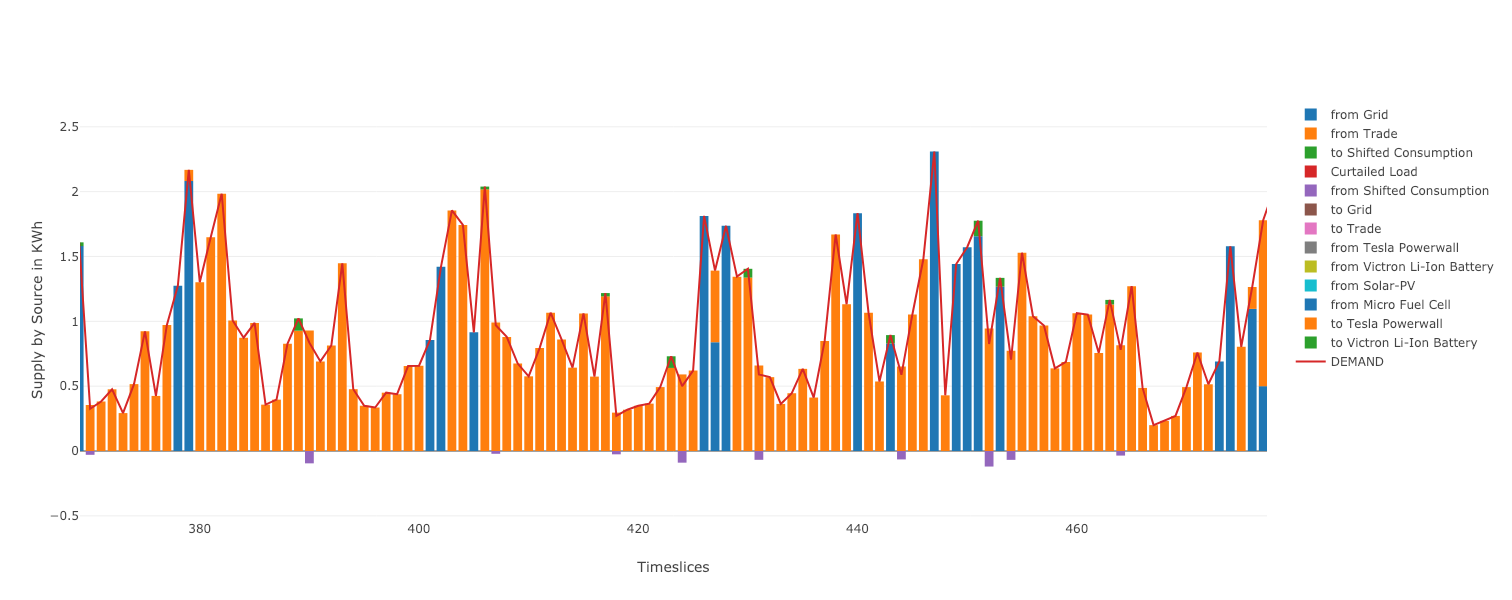
\includegraphics[width=1\textwidth]{pictures/RES_6_DISC.png}
	\caption{A household without generation under an all-discrete constraint during winter}
	\label{commercial_dispatch_base}
	\flushleft\quad\quad\footnotesize{Source: Own Model User Interface}
\end{figure}	


 
\newpage
\chead{\textit{Discussion and Conclusion}}	
\section{Discussion and Conclusion}
Although the sensitivity analysis showed the model result to be quite robust, there are weaknesses to point out: The cost computation is simplified and does not take into account borrowing rates and does not discount future earnings. The results rather reflects a situation in which all equipment is leased and in which interest rates on this leasing contract are negligible. While this is very close to the truth in most of Europe and the U.S., it is still a minor distortion and a major one anywhere else.\\\\
Another weakness is the modeling approach itself. By its very nature LP assumes perfect knowledge of the input parameters involved. This includes all parameters describing demand and supply, which in reality cannot be known at the point of an investment decision. Futhermore dispatch decisions in an LP are also made with perfect knowledge of the future, so every time storage is filled or demand shifted, the perfect amount is certain, which of course also is not the case in a real scenario. This affects only dispatch decisions with an impact on future dispatch decisions however, which our base case does not make a lot of, since it does not have any storage. As a result, the fact that the results arrived at are the product of an LP should only imply a minor advantage in investment optimality, since this can be predicted with quite high accuracy by means of statistics, and in dispatch optimality, since demand shifting is the only dispatch method utilized, which is impacted by perfect foresight. Furthermore demand shifting is mostly utilized for only one hour into the future, for which quite accurate forecasting tools are available, further reducing the information disadvatage of a real life scenario.\\\\
Any minor inaccuracies aside the model results clearly conclude that a microgrid, as described in the base case, if regulatorily feasable, would be highly profitable, with a margin of over 0.13 \euro per KWh. The sensitivity analysis further shows, that even under significant deteroration of some of the assumptions made the margin still remains higher than 0.10 \euro per KWh. There is however some uncertainty involved as being razed by RWE in 2023 would signicantly worsen the profitability of the system. \\
To the question regarding the bigger picture of decentralization, the answer is less clear: While clearly profitable in the context of German electricity retail prices, the generation costs of 0.164 \euro per KWh are still significantly higher than the current generation costs included in the retail price of 0.067 \euro per KWh \cite{Monitoringbericht20182018}. This would conclude, that decentralized generation is still far off, when it comes to large scale competitiveness, it however leaves out of consideration some important factors: First, there is an addtional cost of 0.0719 \euro per KWh incurred by transmission, when buying electricity \cite{Monitoringbericht20182018}. 
In a decentralized scenario of 94 percent autarky, as exhibited in the base results, these costs would most likely be vastly smaller, if at all significant. This brings us to a total of 0.1389 \euro per KWh which is signifcantly closer to the 0.164 \euro result of the base case. Secondly, there is another 0.0917 \euro of levies (excluding taxes) included in the retail price, the majority of which is used to subsidize renewable generation \cite{Monitoringbericht20182018}. Still the present German electricity mix is much dirtier, than the one used in the microgrid of the base case, which consists only of solar and higly efficient natural gas generation. 
Taking this 'power quality' consideration into account the total price of equivalent electricty delivered by a centralized system is (at least in Germany) closer to 0.2305 \euro, which is actually significantly higher than even the results reached in the sensitivity analysis. Furthermore it does not even take into account the heat output of the fuel cells, which can be used without losses for heating water etc. \\
	In addition, it is highly likely, that a major uptake of decentralized generation methods would reduce investment costs, especially of fuel cells, further bringing down the estimated price of electricity. \\
	Of course a decentralized system would incur other costs, as a rudimentary grid would still be needed and industry would possibly suffer from the loss of access to subsidized electricity. \todo{reference eeg umlage}
	Overall though, the results arrived at in this case study suggest a bright future for decentralized generation systems, as they close, or even have closed the cost gap to current centralized ones.

\newpage
\chead{\textit{Appendix}}	

\section{Appendix}
\subsection{Literature Review}
The used search String was:  [microgrid AND (optimization OR opimisation) AND linear programming]
\\
The used databases are ScienceDirect, IEEE Xplore and Google Scholar.
\\
The original dataset consistet of 300 publication of which 275 remained after duplicates where merged.
\\
The search string for the Abstract Keyword Search was [(microgrid OR micro-grid OR off-grid) AND (optimization OR optimisation OR optimise OR optimal OR optimally) AND (linear programming OR linear program OR mixed integer)
\\
After the abstract keyword search was conducted 106 publications remained.
\\
The inclusion criteria were:
\begin{enumerate}
	\item An optimization model is employed.
	\item There is some discussion about the design of the model.
	\item The objective of the model is the optimization of design or dispatch of a single microgrid.
	\item There is some sort of case study conducted.
\end{enumerate}
The exclusion criteria were:
\begin{enumerate}
	\item The publication is not in English language.
	\item The full text is not obtainable for this author with reasonable effort.
	\item The publication is a Work-In-Progress / Conference Paper version of a publication published in a journal and also included in this dataset.
	\item The mathematical model designed is non-linear.
	\item The mathematical model designed only considers a specific aspect of dispatch or design, not the entirety.
	\item The mathematical model is mostly focused on heat generation/distribution rather than electricity.
\end{enumerate}
After the filtering by inclusion and exclusion criteria 58 publications remained.

% weitere Dokumente einfügen mit den gleichen zwei Befehlen

%\nocite{*}	
\newpage								% gibt zum Testen des Literaturverzeichnisses alle Bibeinträge aus
\chead{\textit{References}}				    % siehe oben 
\renewcommand\refname{Literature}			% in Literaturverzeichnis umbenennen
\printbibliography
%[heading=bibintoc]
\end{document}
